% This is the Reed College LaTeX thesis template. Most of the work
% for the document class was done by Sam Noble (SN), as well as this
% template. Later comments etc. by Ben Salzberg (BTS). Additional
% restructuring and APA support by Jess Youngberg (JY).
% Your comments and suggestions are more than welcome; please email
% them to cus@reed.edu
%
% See https://www.reed.edu/cis/help/LaTeX/index.html for help. There are a
% great bunch of help pages there, with notes on
% getting started, bibtex, etc. Go there and read it if you're not
% already familiar with LaTeX.
%
% Any line that starts with a percent symbol is a comment.
% They won't show up in the document, and are useful for notes
% to yourself and explaining commands.
% Commenting also removes a line from the document;
% very handy for troubleshooting problems. -BTS

% As far as I know, this follows the requirements laid out in
% the 2002-2003 Senior Handbook. Ask a librarian to check the
% document before binding. -SN

%%
%% Preamble
%%
% \documentclass{<something>} must begin each LaTeX document
\documentclass[12pt,twoside]{reedthesis}
% Packages are extensions to the basic LaTeX functions. Whatever you
% want to typeset, there is probably a package out there for it.
% Chemistry (chemtex), screenplays, you name it.
% Check out CTAN to see: https://www.ctan.org/
%%
\usepackage{graphicx,latexsym}
\usepackage{amsmath}
\usepackage{amssymb,amsthm}
\usepackage{longtable,booktabs,setspace}
\usepackage{chemarr} %% Useful for one reaction arrow, useless if you're not a chem major
\usepackage[hyphens]{url}
% Added by CII
\usepackage{hyperref}
\usepackage{lmodern}
\usepackage{float}
\floatplacement{figure}{H}
% Thanks, @Xyv
\usepackage{calc}
% End of CII addition
\usepackage{rotating}

% Next line commented out by CII
%%% \usepackage{natbib}
% Comment out the natbib line above and uncomment the following two lines to use the new
% biblatex-chicago style, for Chicago A. Also make some changes at the end where the
% bibliography is included.
%\usepackage{biblatex-chicago}
%\bibliography{thesis}


% Added by CII (Thanks, Hadley!)
% Use ref for internal links
\renewcommand{\hyperref}[2][???]{\autoref{#1}}
\def\chapterautorefname{Chapter}
\def\sectionautorefname{Section}
\def\subsectionautorefname{Subsection}
% End of CII addition

% Added by CII
\usepackage{caption}
\captionsetup{width=5in}
% End of CII addition

% \usepackage{times} % other fonts are available like times, bookman, charter, palatino

% Syntax highlighting #22

% To pass between YAML and LaTeX the dollar signs are added by CII
\title{Short-Term Price Elasticities of Heating Demand: A Statistical Analysis of Energy Billing Data in Germany}
\author{Marc Blauert}
% The month and year that you submit your FINAL draft TO THE LIBRARY (May or December)
\date{2022-04-04}
\division{Albrecht Daniel Thaer-Institute}
\advisor{Prof.~Dr.~Karsten Neuhoff}
\institution{Humboldt University of Berlin}
\degree{Master of Science}
%If you have two advisors for some reason, you can use the following
% Uncommented out by CII
\altadvisor{Prof.~Dr.~Tobias Krüger}
% End of CII addition

%%% Remember to use the correct department!
\department{Integrated Natural Resource Management (INRM)}
% if you're writing a thesis in an interdisciplinary major,
% uncomment the line below and change the text as appropriate.
% check the Senior Handbook if unsure.
%\thedivisionof{The Established Interdisciplinary Committee for}
% if you want the approval page to say "Approved for the Committee",
% uncomment the next line
%\approvedforthe{Committee}

% Added by CII
%%% Copied from knitr
%% maxwidth is the original width if it's less than linewidth
%% otherwise use linewidth (to make sure the graphics do not exceed the margin)
\makeatletter
\def\maxwidth{ %
  \ifdim\Gin@nat@width>\linewidth
    \linewidth
  \else
    \Gin@nat@width
  \fi
}
\makeatother

% From {rticles}
\newlength{\csllabelwidth}
\setlength{\csllabelwidth}{3em}
\newlength{\cslhangindent}
\setlength{\cslhangindent}{1.5em}
% for Pandoc 2.8 to 2.10.1
\newenvironment{cslreferences}%
  {}%
  {\par}
% For Pandoc 2.11+
% As noted by @mirh [2] is needed instead of [3] for 2.12
\newenvironment{CSLReferences}[2] % #1 hanging-ident, #2 entry spacing
 {% don't indent paragraphs
  \setlength{\parindent}{0pt}
  % turn on hanging indent if param 1 is 1
  \ifodd #1 \everypar{\setlength{\hangindent}{\cslhangindent}}\ignorespaces\fi
  % set entry spacing
  \ifnum #2 > 0
  \setlength{\parskip}{#2\baselineskip}
  \fi
 }%
 {}
\usepackage{calc} % for calculating minipage widths
\newcommand{\CSLBlock}[1]{#1\hfill\break}
\newcommand{\CSLLeftMargin}[1]{\parbox[t]{\csllabelwidth}{#1}}
\newcommand{\CSLRightInline}[1]{\parbox[t]{\linewidth - \csllabelwidth}{#1}}
\newcommand{\CSLIndent}[1]{\hspace{\cslhangindent}#1}

\renewcommand{\contentsname}{Table of Contents}
% End of CII addition

\setlength{\parskip}{0pt}

% Added by CII

\providecommand{\tightlist}{%
  \setlength{\itemsep}{0pt}\setlength{\parskip}{0pt}}

\Acknowledgements{
People I need to thank: Franziska, Till, Abteilung beim DIW --\textgreater{} Bereitstellung Daten, Betreuer.
}

\Dedication{

}

\Preface{

}

\Abstract{
The preface pretty much says it all.

\par

Second paragraph of abstract starts here.
}

	\usepackage{setspace}\onehalfspacing
 \usepackage{float}
 \floatplacement{figure}{H}
	\usepackage{booktabs}
 \usepackage{longtable}
 \usepackage{array}
 \usepackage{multirow}
 \usepackage{wrapfig}
 \usepackage{float}
 \usepackage{colortbl}
 \usepackage{pdflscape}
 \usepackage{tabu}
 \usepackage{threeparttable}
 \usepackage{threeparttablex}
 \usepackage[normalem]{ulem}
 \usepackage{makecell}
 \usepackage{xcolor}
% End of CII addition
%%
%% End Preamble
%%
%

\DeclareUnicodeCharacter{2212}{-}
\begin{document}

% Everything below added by CII
  \maketitle

\frontmatter % this stuff will be roman-numbered
\pagestyle{empty} % this removes page numbers from the frontmatter
  \begin{acknowledgements}
    People I need to thank: Franziska, Till, Abteilung beim DIW --\textgreater{} Bereitstellung Daten, Betreuer.
  \end{acknowledgements}

  \hypersetup{linkcolor=black}
  \setcounter{secnumdepth}{2}
  \setcounter{tocdepth}{2}
  \tableofcontents

  \listoftables

  \listoffigures
  \begin{abstract}
    The preface pretty much says it all.

    \par

    Second paragraph of abstract starts here.
  \end{abstract}

\mainmatter % here the regular arabic numbering starts
\pagestyle{fancyplain} % turns page numbering back on

\setlength{\parskip}{6pt} %mblauert, added to see if one can add a skip between paragraphs in the text

\hypertarget{introduction}{%
\chapter{Introduction}\label{introduction}}

\hypertarget{background}{%
\section{Background}\label{background}}

Residential energy demand of private households accounted for 20.2\% of the overall primary energy consumption in Germany in 2020 (\protect\hyperlink{ref-ageb21}{AGEB, 2021}). In turn, 68.1\% of this 20.2\% was used for the purpose of space heating (\protect\hyperlink{ref-rwi21}{RWI, 2021}). Thus, space heating accounts for the largest share of primary energy consumption by private households in their homes. Far exceeding other categories of energy consumption such as hot water generation (16.1\%), process heat (6.0\%), room cooling, information technology, or lighting (all below 5\%) (\protect\hyperlink{ref-rwi21}{RWI, 2021}). Furthermore, the two purposes of space heating and hot water supply continue to predominantly rely on energy from fossil sources. In 2020, 80.1\% of the energy used for space heating came from either natural gas (45.4\%), fuel oil (24.5\%), or district heating (10.1\%)\footnote{Which is at present also to almost 90\% generated from fossil fuels (natural gas or coal) or waste incineration (\protect\hyperlink{ref-destatis18}{DESTATIS, 2018}).} (\protect\hyperlink{ref-rwi21}{RWI, 2021}). These figures convey two messages. First, that the level of energy used for space heating strongly determines the total energy demand in the residential buildings sector. And secondly, that space heating is also the largest source of greenhouse gas (GHG) emissions in the residential buildings sector due to its generation from fossil fuels.

Since 1995, GHG emissions in the building sector in Germany have fallen by 34 \% (\protect\hyperlink{ref-erk20}{ERK, 2020}). This effect is mainly due to lower primary energy consumption through better insulation of the building stock and more efficient heating technologies. In addition, there is an overall lower emission intensity as a result of fuel switching (\protect\hyperlink{ref-erk20}{ERK, 2020}). At the population level, however, these efficiency gains at the household level are partly offset by countervailing effects such as the increase in the number of apartments (smaller average household size) as well as the increase in average living space (\protect\hyperlink{ref-bmwi21}{BMWi, 2021}). Furthermore, much of the efficiency gains on the unit-level were already realized in the 1990s and 2000s. For the last decade, on the other hand, several independent data sources indicate that primary energy consumption per square meter in buildings in Germany has largely stagnated when the effective consumption values are adjusted for spatial and temporal differences in climatic conditions (\protect\hyperlink{ref-bmwi21}{BMWi, 2021}; \protect\hyperlink{ref-stede_etal20}{Stede, Schütze, \& Wietschel, 2020}; \protect\hyperlink{ref-techem19}{Techem, 2019}).

The recent rates of energy consumption and associated GHG emissions in the residential buildings sector therefore not yet reflect the trajectory needed to achieve ambitious climate targets at national and European level, which -- in line with the Paris Agreement -- aim to limit global warming to 1.5 or well below 2 degrees Celsius by 2100. For Germany, the latest amendment of the national Federal Climate Change Act 2021 (Bundes-Klimaschutzgesetz, KSG)\footnote{Federal Climate Change Act of 12 December 2019 (Federal Law Gazette I, p.~2513), as last amended by Article 1 of the Act of 18 August 2021 (Federal Law Gazette I, p.~3905).} stipulates that GHG emissions must reach net-zero in 2045. In addition, the interim target for 2030 was set at a 65\% reduction in GHG emissions compared to the base year 1990 (previously 55\%). Congruently, at the level of the European Union (EU), the Green Deal defines 2050 as the target year to reach net-zero in the whole union (\protect\hyperlink{ref-europeancomission19}{European Comission, 2019}). For the residential buildings sector, achieving these targets requires a comprehensive transformation of energy use, with measures to improve the efficiency of the building stock, demand-side electrification of the remaining energy use, as well as supply-side decarbonisation of energy generation (\protect\hyperlink{ref-hennes_etal21}{Hennes et al., 2021}; \protect\hyperlink{ref-levesque_etal21}{Levesque, Pietzcker, Baumstark, \& Luderer, 2021}).

Basic economic theory relies on the rationale that energy prices represent one of the main drivers for the level of demand for space heat. Against this backdrop, this thesis aims to provide a statistical analysis of price elasticities of heating demand in Germany. Specifically, it is aimed at estimating short-term own-price elasticities of heating demand on the basis of an empirical sample of energy bills in multi-apartment residential buildings in Germany in the period from 2007 to 2019.

\hypertarget{relevance}{%
\section{Relevance of topic}\label{relevance}}

\hypertarget{evaluation-of-price-related-energy-policies}{%
\subsubsection*{Evaluation of price-related energy policies}\label{evaluation-of-price-related-energy-policies}}
\addcontentsline{toc}{subsubsection}{Evaluation of price-related energy policies}

Estimating price elasticities for demand response in the residential buildings sector is relevant for a number of reasons. First, empirical evidence on price elasticities is generally important for evaluating policies that affect the price of energy. Based on elasticity estimates, the economic, distributional and environmental impacts of policy measures can be better understood. In our time, this is especially applicable with regard to the attainment of ambitious climate targets.

One of the most important measures to induce GHG emission reductions in the building sector in Germany is the introduction of a carbon price for heating fuels, which was rolled out in 2021 on the basis of the Fuel Emissions Trading Act (BEHG).\footnote{Fuel Emissions Allowance Trading Act (BEHG) of 12 December 2019 (Federal Law Gazette I p.~2728) as amended by Article 1 of the Act of 3 November 2020 (Federal Law Gazette I p.~2291). Emissions from the building sector have not been subject to carbon pricing in Germany in the past, as they do not fall within the scope of the EU Emissions Trading Scheme (ETS). Besides emissions in the building sector, the BEHG also covers emissions from the transport sector. From 2026 onward the fixed pricing will be superseded by an emission trading system (ETS) with a price corridor.} In general, the introduction of a carbon pricing aims to correct the market failure of the previously unrecognized external effects of greenhouse gas emissions (\protect\hyperlink{ref-aldy_etal10}{Aldy, Krupnick, Newell, Parry, \& Pizer, 2010}; \protect\hyperlink{ref-stiglitz19}{Stiglitz, 2019}). It is expected that the consideration of external effects will have a steering effect on demand through an increased price level. The recently introduced Fuel Emissions Trading Act specifies a fixed price path for the period until 2025. The path rises from an initial price of 25 euros per ton of carbon dioxide (CO\textsubscript{2}) in 2021 to 55 euros per ton of CO\textsubscript{2} in 2025.

Figure \ref{fig:behg} exemplifies the effect of carbon prices for the buildings sector through the BEHG. For gas (Panel A) and oil (Panel B) used for residential space heating, the respective left bar (green) represents the average end consumer prices for the five-year period 2016-2020 from national statistics (\protect\hyperlink{ref-bmwi21}{BMWi, 2021}).\footnote{The 5-year time period (2016-2020) was chosen due to the relatively strong volatility of oil prices in the past years. An exclusive consideration of the price for 2020 would therefore have led to a distortion of the relative price effects. In addition, district heating is not considered here, as most district heating power plants were already subject to carbon pricing under the EU ETS. Only plants with a total combustion capacity of less than 20 megawatts were not previously subject to the EU ETS and will now also be subject to BEHG pricing.} The two middle bars (yellow) show the absolute price effects that occur based on the carbon intensity of the energy carrier in 2021 (25 euro per ton CO\textsubscript{2}) and in 2025 (55 euro per ton CO\textsubscript{2}). The yellow bars are larger for oil due to its higher emission intensity.\footnote{Emission factors for gas (0.201 kg CO\textsubscript{2}e per kWh) and oil (0.266 kg CO\textsubscript{2}e per kWh) were taken from (\protect\hyperlink{ref-uba16}{UBA, 2016}).} Assuming otherwise constant prices, the initial CO\textsubscript{2} price in 2021 would thus lead to a price increase of +0.50 cents (+7.4\%) per kWh gas and +0.66 cents (+13.4\%) per kWh oil. In 2025, the price effects rise to +1.10 cents (+16.3\%) per kWh gas and +1.46 cents (+29.6\%) per kWh oil.
\begin{figure}

{\centering 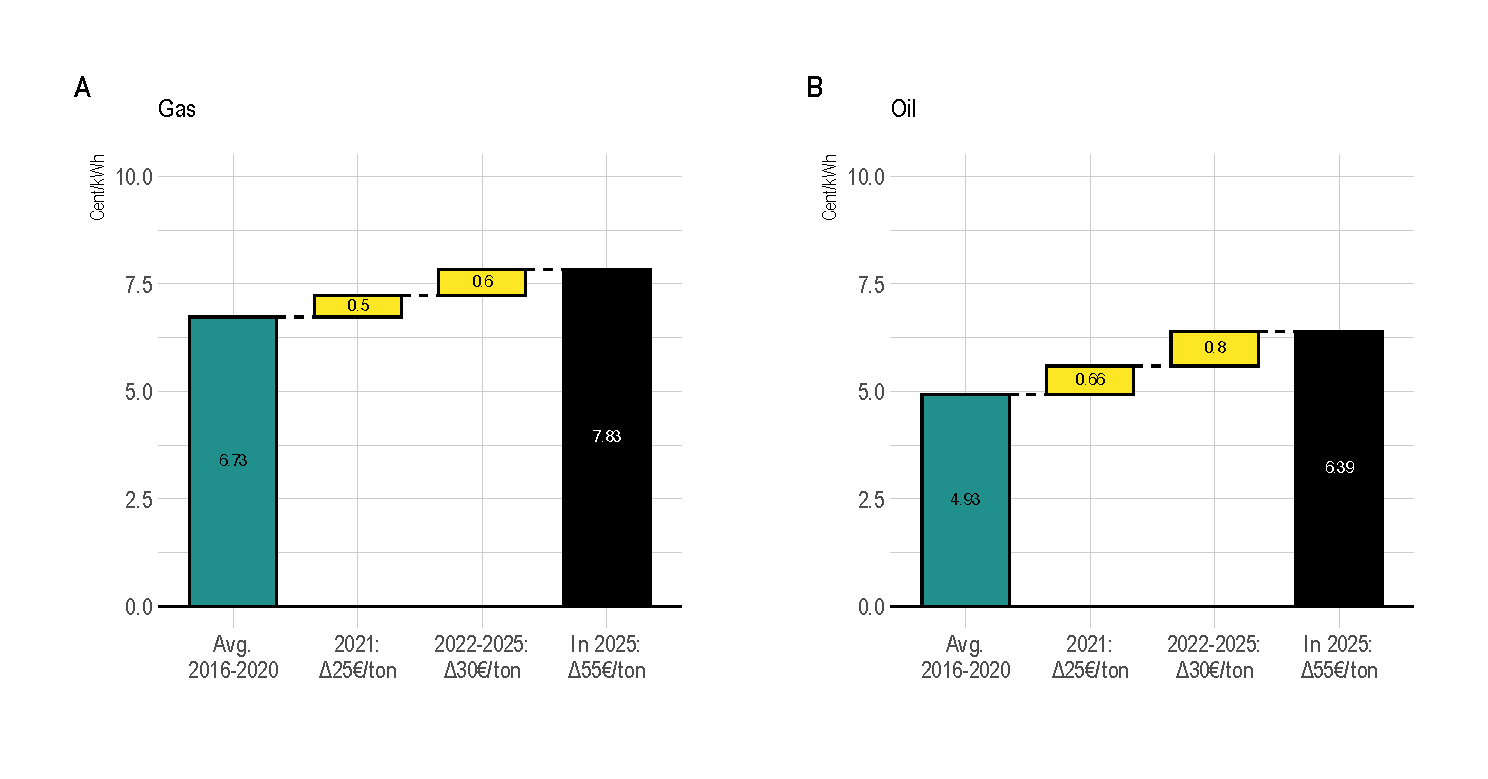
\includegraphics[width=1\linewidth]{figure/price_effect_behg} 

}

\caption[BEHG carbon price effects on gas and oil until 2025]{BEHG carbon price effects on gas and oil until 2025}\label{fig:behg}
\end{figure}
These price figures clearly indicate that relevant steering effects induced by the BEHG are likely to occur already in the next years. Higher price levels driven by the structural price component of carbon pricing can be expected to have two impact channels. The first impact channel are short-term price reactions. Consumers adjust their consumption levels for heating fuels due to higher or lower prices (\protect\hyperlink{ref-alberini_etal11}{Alberini, Gans, \& Velez-Lopez, 2011}). Short-term demand responses are therefore of direct relevance to forecasting building sector energy demand and emission levels in the coming years. The expected effect size of these short-term reactions are reflected by short-term price elasticities of heating demand which will be estimated based on empirical data in this thesis.

The second impact channel, on the other hand, is that higher prices for fossil fuels can be expected to induce long-term steering effects for investments in low-carbon heating technologies and energy efficiency. In the literature, long-term investment decisions driven by mitigation costs potentials are modeled using integrated assessment models (IAMs) for the buildings sector (e.g., \protect\hyperlink{ref-burger_etal19}{Bürger, Hesse, Köhler, Palzer, \& Engelmann, 2019}; \protect\hyperlink{ref-levesque_etal21}{Levesque et al., 2021}). Depending on the model structure, these IAM sector modules are often informed by assumptions on the price elasticities of heating demand as one of their input factor besides other parameters such as the cost of capital or substitution elasticities.\footnote{For a more detailed example of how own price elasticities of demand are taken into account in IAMs, see the model structure description of the ETSAP TIAM model in \protect\hyperlink{ref-loulou_labriet08}{Loulou \& Labriet} (\protect\hyperlink{ref-loulou_labriet08}{2008}). Since IAMs vary in their specific structure and relations other models may consider price elasticities differently.} Therefore, empirical estimates of price elasticities are also important for further analyses in the literature on the second long-term impact channel.

Additionally, the empirical assessment of the demand effect may be particularly important in the current phase of strong energy price increases following from the economic imbalances after the external shock of the COVID-19 pandemic and Russia's war of aggression on Ukraine. While the current price spikes can lead to stronger short-term demand responses, only a fraction of the response is due to the structural component of CO\textsubscript{2} pricing and -- if the effect does not last long enough to trigger significant long-term investments -- would disappear when oil and gas prices might return to lower levels. In order not to overestimate the effect of the structural pricing component of the CO\textsubscript{2} price, empirical estimates from past price reactions could be used to separate the effect into a CO\textsubscript{2} and a commodity price-related element.

\hypertarget{different-types-of-data-to-estimate-elasticities}{%
\subsubsection*{Different types of data to estimate elasticities}\label{different-types-of-data-to-estimate-elasticities}}
\addcontentsline{toc}{subsubsection}{Different types of data to estimate elasticities}

A second line of argument for the relevance of this study is that the existing empirical evidence on the price elasticity of heating demand is based on different types of data sources, but few studies have been conducted on actual billing data.

Studies on the price elasticities of heating demand rely on different types of data sources. For the case of Germany, ex-post statistical analyses for the residential buildings sector use data from social panel surveys (e.g., \protect\hyperlink{ref-rehdanz07}{Rehdanz, 2007}; \protect\hyperlink{ref-schmitz_madlener20}{Schmitz \& Madlener, 2020}; \protect\hyperlink{ref-schulte_heindl17}{Schulte \& Heindl, 2017}). In these studies, household expenditure on heating reported in the survey is usually examined as the relevant variable, but the actual level of energy consumption and energy prices are not observed. This means that, for instance, different energy contract conditions between households may obscure real consumption levels and thus affect the validity of the estimated results. The data available for this thesis is different since the energy bills do provides actual consumption and price data. Other studies using data from energy bills have previously been conducted in the United States (US) (e.g., \protect\hyperlink{ref-auffhammer_rubin18}{Auffhammer \& Rubin, 2018}).

In this context it should be noted that the data sample used in this thesis also has its weaknesses. The data does not observe demand responses at the level of individual households but at the level of multi-household buildings. Yet despite this aggregation of multiple households on the building level, I believe the informative value of estimates to be complementary to estimates from other types of data sources such as social surveys.

\hypertarget{objective}{%
\section{Research questions and objective}\label{objective}}

Against the background of the tightened climate targets, the recently introduced carbon pricing, and the sharp price increases for heating fuels, the question of the price elasticity of heating demand is once again moving to the center of public attention. The aim of this work is to investigate the price elasticity of heating demand in multi-family houses in Germany based on a large-scale sample of energy bills. The guiding research questions for the analysis are:
\begin{itemize}
\tightlist
\item
  How does a change in energy price affect the level of energy consumption?
\item
  What other variables might affect energy consumption and need to be taken into account so that their effects are not falsely attributed to energy prices?
\item
  And, are there potential factors for heterogeneity within the sample that would be obscured when only estimating an overall elasticity?
\end{itemize}
By using energy bills as a data source, the study aims to complement existing studies based on different sources. Furthermore, the period studied is more recent and can therefore complement older studies. Also, the analysis aims not only to estimate an overall elasticity, but also to investigate potential factors for heterogeneity. The statistical analysis aims to use several different modelling approaches, both Frequentist and Bayesian. As far as the author is aware, the Bayesian approach has not been used in previous research in this field. Furthermore, the elasticity estimates from this work may also be relevant for other countries and regions that have comparable conditions to Germany in terms of building stock and energy demand and also face the challenge of decarbonising the building sector in the coming decades. Here, my results would serve as an empirical guide to the short-term demand effects for any kind of price-related policy instrument.

The thesis is structured in six Chapters. While the first Chapter was used to provide an introduction, Chapter \ref{literature} gives an overview on the existing literature on price elasticities of space heating demand. In the following Chapter \ref{methods} the data and methods used for the analysis are laid out. Chapter \ref{results} provides the results of the analysis, which are then discussed in Chapter \ref{discussion}. Chapter \ref{conclusion} provides concluding remarks.

\hypertarget{literature}{%
\chapter{Theory and Literature}\label{literature}}

The objective of this chapter is to provide a short theoretical background on price elasticities as well as an overview of the previous research on price elasticities of heating demand. The text is organized as follows. The first part of the chapter focuses on the theoretical background and also provides a placement of the effects of varying elasticities in connection to heating demand. The second part of the chapter then moves to summarizing the empirical evidence from the literature.

\hypertarget{theory}{%
\section{Price elasticity of demand}\label{theory}}

Elasticities are one of the key concepts in mirco-economic theory. They are used to express the sensibility of one variable to a change in another. The own price elasticity of demand is one type of elasticity. It represents the magnitude of a change in consumption of a good following from a change in its own price (\protect\hyperlink{ref-pindyck_rubinfeld18}{Pindyck \& Rubinfeld, 2018}). Formally, the own price elasticity of demand \(\epsilon\) can be expressed as
\begin{equation}
\epsilon = \frac{\frac{\Delta Q}{Q}}{\frac{\Delta P}{P}} = \frac{P \Delta Q}{Q \Delta P}
\label{eq:ep}
\end{equation}
where \(\Delta P/P\) represents the percentage change in the price \(P\) of a good and \(\Delta Q/Q\) the corresponding percentage change in the quantity \(Q\) demanded of the same good. Due to budget constraints, consumers tend to consume less of a good when its price increases, which implies that under normal conditions the price elasticity of demand is negative. But the responsiveness of the demand reaction may vary across different goods. A common assumption in the econometric literature is that elasticities are constant (\protect\hyperlink{ref-varian10}{Varian, 2010}). Leading to a demand function that can be expressed by
\begin{equation}
Q = AP^{\varepsilon}
\label{eq:demand}
\end{equation}
where \(A\) represents an arbitrary constant and \(\epsilon\) again is the price elasticity of demand. Taking the logarithms of the demand function removes \(\epsilon\) from the exponent and yields
\begin{equation}
ln(Q) = ln(A) + \epsilon \; ln(P)
\label{eq:demand2}
\end{equation}
which can be referred to as the elasticity case and will reappear at a later point, when constructing the regression models to estimate price elasticities from the sample data.

To make the assumption of constant elasticity more intuitive, it seems useful to return to the subject of interest and show the behavior of demand curves for space heating under varying price elasticities of demand. Generally, the literature distinguishes between three different types of elasticities. If the demand response for a good is greater than the change in its price (\(\epsilon < -1\)), it is called price elastic. If the demand response is exactly equal to the change in price (\(\epsilon = -1\)), it is said to be unit-elastic. Finally, if the demand response is smaller than the price change (\(0 > \epsilon > -1\)) -- and therefore indicating a lower responsiveness -- it is called price inelastic (\protect\hyperlink{ref-pindyck_rubinfeld18}{Pindyck \& Rubinfeld, 2018}).\footnote{It should be noted that in the literature the minus of the demand elasticity \(\epsilon\) is sometimes omitted, as it is assumed that it is generally negative. However, I personally find it more intuitive not to do so -- especially when working empirically where positive estimates are a possibility -- and will therefore continue to use the negative values in this thesis.}

Figure \ref{fig:elasticities-conceptual} visually represents these different price elasticities for the demand of space heating.\footnote{Please note that in the graph, energy price as the independent variable is plotted on the horizontal axis and energy demand as the response variable on the vertical axis. I consider this convention -- which is common in most of science -- to be more intuitive than the traditional Marshallian cross diagram in Economics, where the price is plotted on the vertical axis.} To construct the demand curves, a common arbitrary intersection point is chosen for the curves. Specifically, this intersection has a demand value of 130 kilowatt hours (kWh) per square metre (sqm) and a price of 6 cents per kWh. These values can be considered realistic for an average building in Germany, as we will see later in this thesis when working with the sample data.
\begin{figure}

{\centering 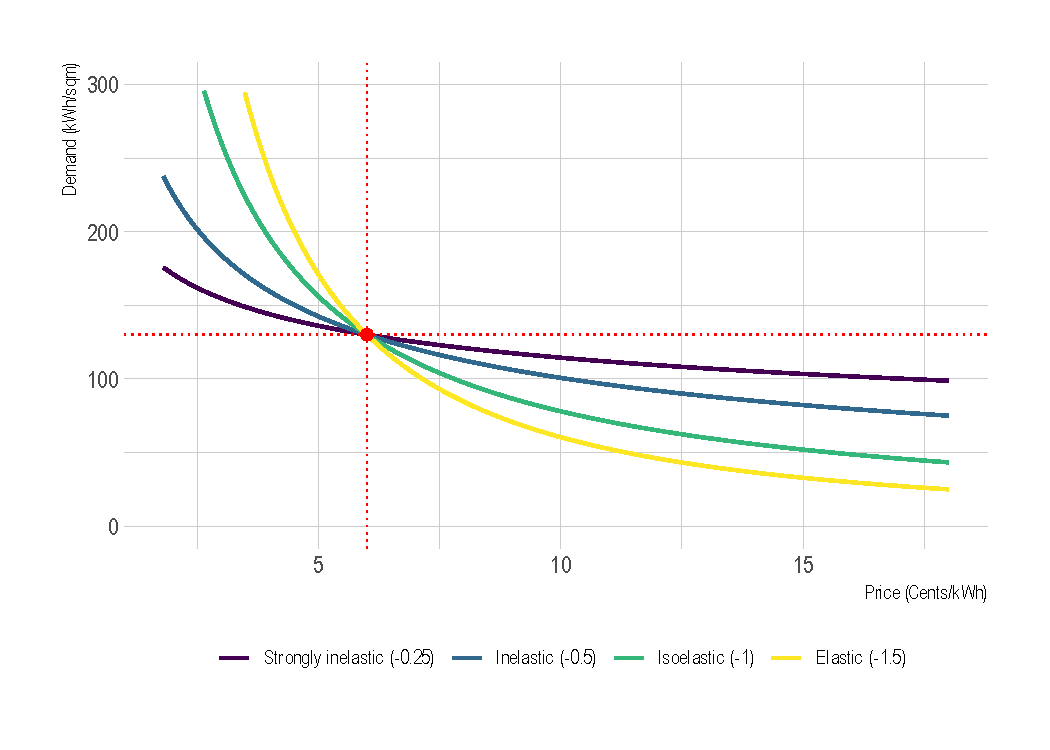
\includegraphics[width=1\linewidth]{figure/elasticities_plot} 

}

\caption{Demand curves with different price elasticities of demand}\label{fig:elasticities-conceptual}
\end{figure}
The graph shows a total of four demand curves. In addition to the unit-elastic curve (\(\epsilon = -1\)), there is also an elastic (\(\epsilon = -1.5\)) and two inelastic (\(\epsilon = -0.25, \epsilon = -0.5\)) demand curves. The special feature of the unit elastic demand curve is that it gives the same result for total expenditure on heating costs for all combinations of price times demand. This is not the case with the other elasticities. First, a look to the right of the intersection (higher prices). In the elastic case (yellow curve), total expenditures fall when the price is higher, which means that households can adjust their demand downwards more. In the opposite, inelastic cases (purple and blue curves), on the other hand, households would reduce their demand less and therefore also have higher total expenditure. Conversely, to the left of the intersection point (lower prices), more elastic demand (yellow curve) leads to a higher level of energy demand and thus also to higher total expenditure than in the inelastic cases (purple and blue curves), where demand changes only gradually.

If we now take a step back and consider what kind of good the demand for space heating represents and what price elasticity of demand one might expect, it seems reasonable to assume that the elasticity is rather inelastic. There are two indications leading to this assumption. First, heating energy is to be regarded as an essential good that is associated with a minimal level of demand -- especially in the winter months. Essential goods tend to follow a more inelastic demand pattern than other types of goods (\protect\hyperlink{ref-gwartney76}{Gwartney, 1976}). Households can only reduce their demand to a certain extent (right side of the intersection), but on the other hand, they do not have a strong rationality for a large increase in heating demand beyond a comfortable level of warmth (left side of the intersection). The second indication for a rather inelastic demand is that due to the dependency on the existing heating system -- especially for the tenant households investigated in this thesis -- there is not really a viable option to substitute space heating from one source with space heating from another.

Another important dimension for distinguishing different price elasticities of demand is time. More precisely, the time that elapses between a price signal and the measurement of the demand response. Here, the literature distinguishes between short-term and long-term price elasticities (also called short- and long-run elasticities) (\protect\hyperlink{ref-pindyck_rubinfeld18}{Pindyck \& Rubinfeld, 2018}). Short-term elasticities are those that are estimated in temporal proximity to the price change -- in this case, that would be the energy price change within a billing year and the associated change in demand in the same period (or in the year after the price change). Long-term elasticities, on the other hand, imply that more time has elapsed for consumers to fully adjust to a price change and also to make long-term investment decisions that would change the overall level of demand (\protect\hyperlink{ref-pindyck_rubinfeld18}{Pindyck \& Rubinfeld, 2018}). For the subject at hand, such decisions may include changes in the isolation of a building or an exchange of the heating system. Thus, long-term demand elasticities tend to be larger than their short-term counterparts (\protect\hyperlink{ref-schmitz_madlener20}{Schmitz \& Madlener, 2020}). Therefore, the two types can be seen as mirroring the two different channels through which a pricing policy can influence consumer behavior (see Section \ref{relevance}).

In the literature, long-term price elasticities are usually estimated using dynamic models, where the elasticity estimated between two periods is only a fraction of the long-term elasticity (e.g., \protect\hyperlink{ref-alberini_etal11}{Alberini et al., 2011}). However, I have chosen follow the example of \protect\hyperlink{ref-schmitz_madlener20}{Schmitz \& Madlener} (\protect\hyperlink{ref-schmitz_madlener20}{2020}) and only estimate short-term elasticities.This is because I believe that the long-term approaches do not apply well to the given context in which I am analyzing a subset of the total residential building segment consisting of rental buildings where households have relatively few opportunities to make long-term adjustments that would significantly affect the energy efficiency or carbon intensity of the energy of their apartments.

\hypertarget{review}{%
\section{Literature review}\label{review}}

The study of the price elasticity of energy demand is a broad field of academic research which also has a long history dating back to the mid-twentieth century (e.g. \protect\hyperlink{ref-cutler41}{Cutler, 1941}; \protect\hyperlink{ref-houthakker51}{Houthakker, 1951}). In the more recent past, as well numerous studies have been published. These studies differ considerably in terms of their focus and design. Several conceptual factors can systematically influence the elasticity estimates. The most important of these factors is the type of energy application analysed: The price responsiveness of household space heating demand has only limited informative value for the price responsiveness of electricity demand or transport fuel demand. The same is true for varying consumer groups: Households are likely to react differently to energy price changes than industrial consumers. Beyond, other conceptual factors which may as well affect estimates are the statistical methods used (time-series analysis, panel analysis, cross-sectional analysis), varying sources of data (national accounts, aggregate sector-level data, micro-data), varying spatial and temporal focus, measurement heterogeneity, and price trends (\protect\hyperlink{ref-csereklyei20}{Csereklyei, 2020}; \protect\hyperlink{ref-miller_alberini16}{Miller \& Alberini, 2016}). While many of the earlier studies either had only a national granularity or, when using micro data, focused predominantly on the US or European countries, a considerable number of studies have also been published recently that cover emerging countries (especially China) as well as other countries.

\textbf{Meta-estimates as first indication of elasticity magnitudes}

To organize this comprehensive body of literature with a wide range of energy applications, meta-studies do serve as a good starting point. The recently published meta-analysis by \protect\hyperlink{ref-labandeira_etal17}{Labandeira, Labeaga, \& López-Otero} (\protect\hyperlink{ref-labandeira_etal17}{2017}) is particularly suitable for this purpose, as it covers a broad spectrum of energy uses and thus goes beyond previous meta-analyses that primarily focus on the elasticity of petrol demand. I will therefore first delve into the aforementioned meta-analysis before turning to a subset of selected studies that take a closer look at the specific issue of price elasticities for space heating demand in the residential buildings sector.

In their analysis, \protect\hyperlink{ref-labandeira_etal17}{Labandeira et al.} (\protect\hyperlink{ref-labandeira_etal17}{2017}) include a total of 428 papers, all published between 1990 and 2016. For the demand of natural gas, they find an average short-term (long-term) price elasticity of -0.18 (-0.57) based on 230 individual estimates. And for heating oil they find a comparable average short-term (long-term) elasticity of -0.19 (-0.54), which, however, is based on only 44 individual estimates (\protect\hyperlink{ref-labandeira_etal17}{Labandeira et al., 2017}). An average elasticity for space heating -- which is generally less focused on in the literature due to its relatively low prevalence -- is not given.

The above average estimates of the price elasticity of demand for gas and oil, however, come with an important caveat. While they are broken down by energy carrier, they are drawn from a wide range of consumer groups. This means that the underlying studies include not only those that examine demand response patterns for residential consumption, but also others that examine these patterns for the commercial building stock and/or the industrial sector. \protect\hyperlink{ref-labandeira_etal17}{Labandeira et al.} (\protect\hyperlink{ref-labandeira_etal17}{2017}) also provide average price elasticities stratified by consumer groups, but these are on the other hand not clustered by energy source. When differentiated along the dimension of consumer groups, they report that the average estimates are slightly higher in the residential household sector (short-term: -0.22; long-term: -0.62) than in the industrial sector (short-term: -0.17; long-term: -0.51), which seems reasonable given that households likely have more ability to change their level of demand than the industrial sector with more fixed production patterns and the ability to forward costs. Overall, however, the average elasticity estimates are all in a similar size range and together convey the message that demand is strongly inelastic in the short-term, confirming the theoretical arguments that energy is an essential good in many applications and also has limited substitutability (see section \ref{theory}).

The meta-estimates are useful in providing a high-level overview. However, as already mentioned, they include estimates from a wide range of energy applications that not necessarily reflect the demand response for the specific application of space heating in residential buildings. Furthermore, they are average estimates which may have the effect of masking discrepancies and variations between studies. Therefore, the following section presents individual studies that explicitly focus on the space heating demand of the residential sector.

\textbf{Selected studies on space heating in the residential buildings sector}

The space heating demand of the residential sector represents a subset of the full literature stream. The selected studies were chosen based on the criteria that they correspond to the focus of this work and are of good quality (peer-reviewed journal articles). A summary of the studies is provided in Table \ref{tab:estimates-literature}.

There are three earlier studies that have a spatial focus on Germany. The first study was conducted by \protect\hyperlink{ref-rehdanz07}{Rehdanz} (\protect\hyperlink{ref-rehdanz07}{2007}), who estimates price elasticities for different energy carriers for residential heating demand. She uses social survey data on household-level heating expenditures from the Socio-Economic Panel (SOEP) in the years 1998 and 2003. Methodologically, a cross-sectional statistical analysis with dummy variables is conducted for the two years -- in other words, no panel structure is used. In contrast to the average meta-estimates presented in the previous section, the study finds that demand for heating oil has a high elasticity of -1.68 to -2.03, depending on the model specification. For gas, the results indicate a less elastic demand between -0.44 and -0.63, also depending on the model used. Therefore the study concludes that the type of fuels can have a strong influence on the price sensitivity of households (\protect\hyperlink{ref-rehdanz07}{Rehdanz, 2007}).
\begin{table}[]
\centering
\caption{Selected studies on the price elasticity of heating demand}
\label{tab:estimates-literature}
\resizebox{\textwidth}{!}{%
\begin{tabular}{@{}llll@{}}
\toprule
\textbf{Study} & \textbf{Type of data used} & \textbf{\begin{tabular}[c]{@{}l@{}}Energy \\ carrier\end{tabular}} & \textbf{\begin{tabular}[c]{@{}l@{}}Short-term\\ price elasticities\end{tabular}} \\ \midrule
 &  &  &  \\
{\ul \textit{Studies within Germany}} &  &  &  \\
\multirow{2}{*}{Rehdanz (2007)} & \multirow{2}{*}{\begin{tabular}[c]{@{}l@{}}Social survey, panel data (SOEP),\\ all types of buildings, 1998 and 2003\end{tabular}} & Gas & -0.44 to -0.63 \\
 &  & Oil & -1.68 to -2.03 \\
Schmitz and Madlener (2020) & \begin{tabular}[c]{@{}l@{}}Social survey, panel data (SOEP), \\ all types of buildings, 1996-2014\end{tabular} & (All) & -0.31 to -0.43 \\
Schulte and Heindl (2017) & \begin{tabular}[c]{@{}l@{}}Social survey, panel data (EVS),\\ all types of buildings, 1993-2008\end{tabular} & (All) & -0.50 \\
 &  &  &  \\
{\ul \textit{Studies outside of Germany}} &  &  &  \\
Alberini et al. (2011) & \begin{tabular}[c]{@{}l@{}}US, household-level social survey, \\ 50 metropolitan areas, panel data, 1995-2007,\\ only single-family homes and duplexes\end{tabular} & Gas & -0.57 to −0.69 \\
Auffhammer and Rubin (2018) & \begin{tabular}[c]{@{}l@{}}US, energy billing data, household-level, \\ only California, panel data, 2003-2014\end{tabular} & Gas & -0.17 to -0.23 \\
\begin{tabular}[c]{@{}l@{}}Leth-Petersen and \\ Togeby (2001)\end{tabular} & \begin{tabular}[c]{@{}l@{}}Denmark, apartment-block level (\textgreater{}1,500 sqm),\\ panel data, 1984-1995\end{tabular} & Oil & -0.08 \\
 &  & District heating & -0.02 \\
\multirow{2}{*}{Meier and Rehdanz (2010)} & \multirow{2}{*}{\begin{tabular}[c]{@{}l@{}}UK, household-level social survey,\\ panel data 1991-2005\end{tabular}} & Gas & -0.34 to -0.56 \\
 &  & Oil & -0.40 to -0.49 \\
Metcalf and Hassett (1999) & \begin{tabular}[c]{@{}l@{}}US, household-level, panel data, \\ 1984, 1987 and 1990\end{tabular} & Gas & -0.48 to -0.71 \\ \bottomrule
\end{tabular}%
}
\end{table}
In a more recent study, also based on the SOEP social survey data but covering a more comprehensive time period between 1996 and 2014, \protect\hyperlink{ref-schmitz_madlener20}{Schmitz \& Madlener} (\protect\hyperlink{ref-schmitz_madlener20}{2020}) find a price elasticity of heating and hot water demand of -0.31 to -0.43, depending on model specifications. They do not differentiate the elasticities by energy carrier. The price elasticities are derived from household expenditure elasticities, as demand is not directly observed. In contrast to \protect\hyperlink{ref-rehdanz07}{Rehdanz} (\protect\hyperlink{ref-rehdanz07}{2007}), the study uses a panel structure where observations are clustered by household and year using fixed effects. This produces much lower price elasticity estimates, which are more consistent with the meta-estimates presented in the previous section. Moreover, the study discovers that price elasticity is heterogeneous across different socio-economic groups. Given the household-level information at their disposal, they find that higher-income households are less sensitive to energy price changes than lower-income households. Likewise, homeowners show less sensitivity than renters (\protect\hyperlink{ref-schmitz_madlener20}{Schmitz \& Madlener, 2020}).

Also for Germany, \protect\hyperlink{ref-schulte_heindl17}{Schulte \& Heindl} (\protect\hyperlink{ref-schulte_heindl17}{2017}) investigate the price and expenditure elasticities of private energy demand in Germany between 1993 and 2008. For their analysis, they use survey data from the \emph{Einkommens- und Verbrauchsstichprobe (EVS)} and analyse them with a demand system approach (in particular, they estimate a quadratic expenditure system). For space heating, they find an own-price elasticity of -0.50 across all households. They further observe that the price elasticity changes with the level of total household expenditure, with households in higher expenditure strata reacting more strongly to price changes (\protect\hyperlink{ref-schulte_heindl17}{Schulte \& Heindl, 2017}). Put differently, this means that following an increase in price level low income households tend to lower energy demand to a lesser extent as compared to households with a higher income. Thus, in relation to the income dimension the results must be understood as contradictory to those of \protect\hyperlink{ref-schmitz_madlener20}{Schmitz \& Madlener} (\protect\hyperlink{ref-schmitz_madlener20}{2020}).

All three studies on Germany rely on data from household-level social surveys. Therefore, the studies take a strong perspective on the impact of household income on energy price sensitivity. As the data for this study is aggregated at the building-level and not at the household-level, however, the focus of this thesis is to some extent different. The focus is rather on the overall price response based on actual price and consumption values, which are not available in the social surveys, and on the response in interaction with other characteristics and changes at the building level.

Besides the studies focusing on Germany, Table \ref{tab:estimates-literature} also reports the evidence from five selected international studies focusing on the price elasticities of space heating demand. \protect\hyperlink{ref-alberini_etal11}{Alberini et al.} (\protect\hyperlink{ref-alberini_etal11}{2011}) examine household demand for gas (and electricity) in single-family homes and duplexes using household-level social survey data in 50 metropolitan areas in the United States (US) over the period 1995-2007. As a modelling approach, they use static and dynamic panel models. For the static models reflecting the approach taken in this thesis, they find an own price elasticity of private gas demand between -0.57 and -0.69, depending on the model specification. These estimates are in their magnitude comparable to the results of an earlier study by \protect\hyperlink{ref-metcalf_hassett99}{Metcalf \& Hassett} (\protect\hyperlink{ref-metcalf_hassett99}{1999}) who use the 1984, 1987 and 1990 waves of the US Residential Energy Consumption Survey (RECS) to examine homeowners' investments in energy efficiency measures and as part of their study find price elasticities of residential gas demand to range between −0.48 and −0.71. In contrast to these estimates, a recent study by \protect\hyperlink{ref-auffhammer_rubin18}{Auffhammer \& Rubin} (\protect\hyperlink{ref-auffhammer_rubin18}{2018}) finds that the short-term price elasticity of residential gas demand is even more inelastic, ranging from -0.17 to -0.23, not for the whole US but for California in particular. The study by \protect\hyperlink{ref-auffhammer_rubin18}{Auffhammer \& Rubin} (\protect\hyperlink{ref-auffhammer_rubin18}{2018}) is especially interesting for this thesis because it is the only one that also uses energy billing data. The data analysed covers the period 2003-2014 and consists of monthly energy bills at the household-level. So although the type of data source used to derive the estimates is the most similar to the approach taken in this thesis, there are still two relevant differences: firstly, gas tariffs in the US nay change monthly rather than annually, as is the case in the German dataset used for this analysis, and secondly, the data in \protect\hyperlink{ref-auffhammer_rubin18}{Auffhammer \& Rubin} (\protect\hyperlink{ref-auffhammer_rubin18}{2018}) relates to individual households rather than the aggregate building-level.

In addition to these three studies focusing on the US, Table \ref{tab:estimates-literature} also contains the results of a Danish study by \protect\hyperlink{ref-leth-petersen_togeby01}{Leth-Petersen \& Togeby} (\protect\hyperlink{ref-leth-petersen_togeby01}{2001}). They use a panel data approach and analyse data from the period 1984-1995. Interestingly, they also use the building-level as the level of analysis. More specifically, they study apartment buildings with a base area of more than 1,500 square meters (sqm) in Denmark. As an empirical strategy, they rely on fixed effects models. As a result, they find very inelastic demand responses for space heating. For oil, the short-term price elasticity is found to be -0.08 and for district heating as low as -0.02, meaning almost no demand response to a changing price at all. Another study by \protect\hyperlink{ref-meier_rehdanz10}{Meier \& Rehdanz} (\protect\hyperlink{ref-meier_rehdanz10}{2010}) looks at the United Kingdom (UK) and analyses a household-level social survey panel for the 15-year period 1991-2005. For their model they use a log-linear approach. They find that the short-term price elasticity of demand for gas ranges from -0.34 to -0.56, depending on the specification. For residential oil demand, the results are in the same order of magnitude, but narrower, between -0.40 and -0.49. In addition, they find that the type of occupant is a relevant dimension for a different price responsiveness. While renters adjusted their demand level more, homeowners showed a more inelastic response.

\textbf{Synthesis of estimates from the literature}

When summarizing the literature on the price elasticity of residential space heating demand presented previously, commonalities and differences emerge. The most important commonality is that the price elasticity of energy demand in general and household space heating demand in particular is inelastic in almost all empirical estimations. But at the level of individual studies, differences in the magnitude of the estimates persist. While the meta-results by \protect\hyperlink{ref-labandeira_etal17}{Labandeira et al.} (\protect\hyperlink{ref-labandeira_etal17}{2017}) as well as a number of individual studies indicate a strongly inelastic demand response (e.g. \protect\hyperlink{ref-auffhammer_rubin18}{Auffhammer \& Rubin, 2018}; \protect\hyperlink{ref-leth-petersen_togeby01}{Leth-Petersen \& Togeby, 2001}), other individual studies still indicate an inelastic but stronger demand response (e.g., \protect\hyperlink{ref-alberini_etal11}{Alberini et al., 2011}; \protect\hyperlink{ref-meier_rehdanz10}{Meier \& Rehdanz, 2010}; \protect\hyperlink{ref-metcalf_hassett99}{Metcalf \& Hassett, 1999}; \protect\hyperlink{ref-rehdanz07}{Rehdanz, 2007}; \protect\hyperlink{ref-schmitz_madlener20}{Schmitz \& Madlener, 2020}; \protect\hyperlink{ref-schulte_heindl17}{Schulte \& Heindl, 2017}). These differences in magnitude may be partly due to the different local and temporal conditions of the studies or due to differences in the data and methodology. Such aspects may also include behavioral aspects related to a specific population. Figure \ref{fig:literature-estimates-plot} graphically represents the short-term elasticity estimates from Table \ref{tab:estimates-literature}. As a synthesis, all studies that focused on Germany found somewhat more sensitive price elasticities ranging from -0.3 to -0.6.\footnote{Note that the extreme results of \protect\hyperlink{ref-rehdanz07}{Rehdanz} (\protect\hyperlink{ref-rehdanz07}{2007}) for the carrier oil, which come only from a cross-sectional regression analysis, are omitted here. Since only two isolated periods are considered, these results must be considered more prone to extreme results than is the case with a longer panel.} And also most estimates from other countries can be allocated to that range of price sensitivity.
\begin{figure}

{\centering 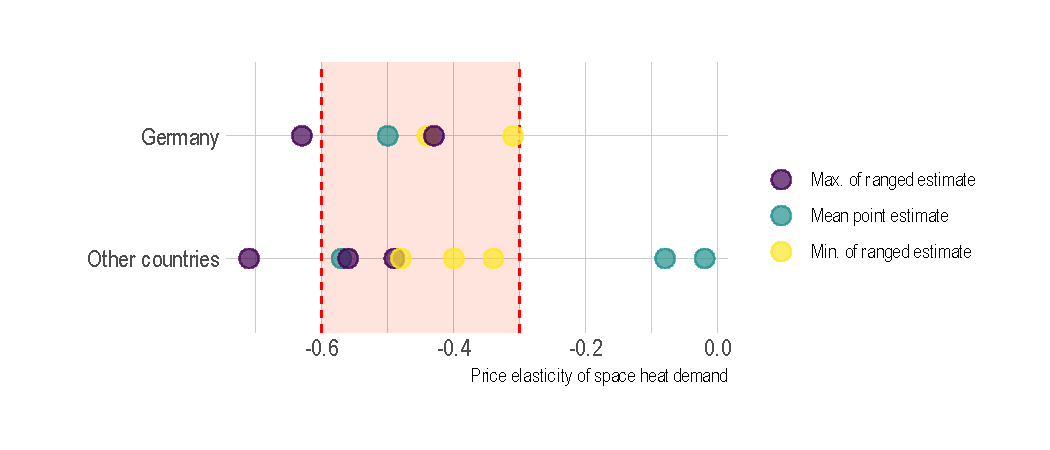
\includegraphics[width=1\linewidth]{figure/plot_literature_estimates} 

}

\caption{Price elasticity of space heat demand estimates from individual studies}\label{fig:literature-estimates-plot}
\end{figure}
Importantly, another common feature that links all the individual studies presented is that they do not focus on one-off extreme price shocks as an identification strategy, but on gradual price developments. They are mostly built around a panel data set covering a longer period of time. The period examined in this study also covers more than a decade with rather gradual price developments. This should therefore be considered an important condition that facilitates the comparability of the results of this study with the estimates presented in the literature.

\hypertarget{conceptual-model}{%
\section{Conceptual model development}\label{conceptual-model}}

In the previous two subsections, the theory around price elasticities of demand (see section \ref{theory}) and evidence from the prior literature (see section \ref{review}) in the context of space heating demand have been presented. To complete this foundation, this subsection uses the theory, but more importantly the approaches of prior studies, to identify relevant variables in the relationship between space heating demand and energy price. The aim is to create a conceptual model, which will then be translated into a statistical model and empirically examined in the further course of this thesis.

\textbf{Price elasticity}

The starting point for the conceptual model is the relationship between space heating demand and energy price. Here, the basic assumption from the theory of price and demand is that the demand for space heating is influenced by the energy price. When the price goes up, demand moves down along the demand curve and vice versa (see Figure \ref{fig:elasticities-conceptual}). Transferred to a statistical terminology this implies that space heat demand is the response variable of a model and energy price the main explanatory variable. To support the development of the conceptual model visually, Figure \ref{fig:dag} depicts it as a directed acyclic graph (DAG).\footnote{Please note that the relationships between space heat demand and the variables used to explain it are of relevance here. Other relationships among explanatory variables are hinted at for the sake of completeness, but are not explicitly examined in the course of the thesis.} In the center, the space heat demand is shown, the variance of which is to be explained (yellow bubble). Since the effect of energy price (purple bubble) on space heating demand is to be regarded as the price elasticity, it is marked with a red arrow.
\begin{figure}

{\centering 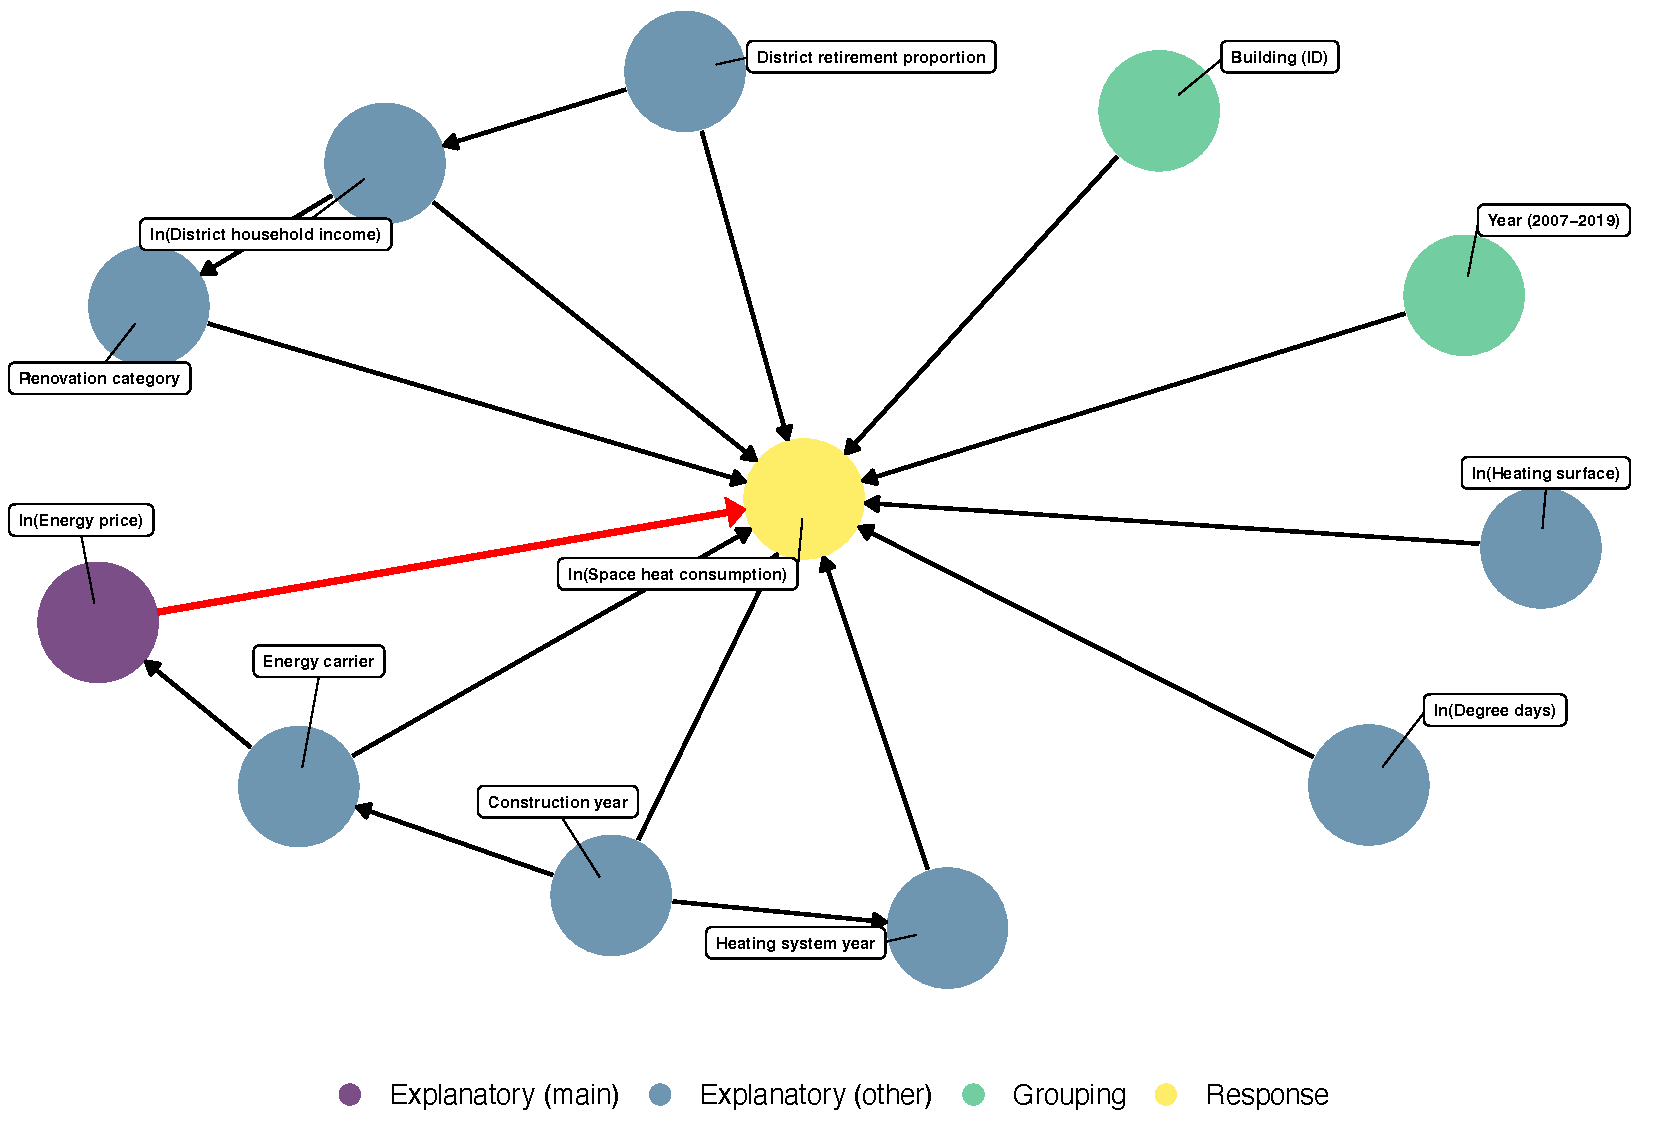
\includegraphics[width=1\linewidth]{figure/conceptual_dag_red} 

}

\caption[Conceptual model as directed acyclic graph]{Conceptual model as directed acyclic graph}\label{fig:dag}
\end{figure}
In addition to the energy price, there are a whole range of other variables that may influence the level of space heating demand. These are shown in the DAG as additional explanatory variables (blue bubbles) and as grouping variables (green bubbles). In order to establish the additional variables relevant for the model, I used a structured procedure. First, I used the recent work of \protect\hyperlink{ref-schmitz_madlener20}{Schmitz \& Madlener} (\protect\hyperlink{ref-schmitz_madlener20}{2020}) as a basis to create a list of potential variables. Secondly, I used the additional studies presented in Section \ref{review} to cross-validate their relevance and to screen for further variables. This structured approach leads to the variables presented in the following.

\textbf{Climatic condition}

Firstly, the consideration of the local climatic condition in a billing period is of importance, as it can have a strong influence on the heating demand (\protect\hyperlink{ref-hesse20}{Heße, 2020}). In the individual studies presented in Section \ref{review} climatic conditions are always considered. Usually, climatic conditions are approximated by the outdoor temperature, measured in (heating) degree days. In line with \protect\hyperlink{ref-vdi13}{VDI} (\protect\hyperlink{ref-vdi13}{2013}), degree days in this study are defined as the temperature difference between a mean room temperature of 20°C and the daily mean of the outdoor temperature, provided it is below the heating limit of 15°C.\footnote{It should be noted that the definition of degree days used here differs from the internationally frequently used definition of heating degree days (HDD), which is calculated by difference between the average outdoor temperature below a heating threshold over time -- regardless of an additionally defined room temperature. In this thesis, the VDI based definition of degree days was chosen, as this is the common methodology in Germany, which is also used, for example, to create a comparable scoring for building energy performance certificates (see \protect\hyperlink{ref-halbig_namyslo14}{Halbig \& Namyslo} (\protect\hyperlink{ref-halbig_namyslo14}{2014})).} The intuition is that with lower mean outdoor temperatures, transmission heat losses increase and thus the demand for space heating increases to compensate for those heat losses. Lower mean outdoor temperatures are associated with a higher aggregated number of degree days in a period. Thus, one would expect a higher space heating demand when the degree days in an annual heating cycle are higher and vice versa. Varying degree days may occur on a temporal (one year is warmer/cooler than another) but also on a spatial scale (places at higher altitudes or in the interior of the continent have structurally lower temperatures).

\textbf{Building-level characteristics}

In addition, various building characteristics are included in the model as additional explanatory variables. Firstly, the size of a building can influence the heat demand, as in larger buildings the ratio between the external surface of the building and the heating surface decreases and thus the relative share of transmission heat losses per unit of heating surface is lower correspondingly. Therefore, it can be assumed that in buildings with a larger heating surface -- which approximates the size of a building -- the space heating demand per unit would be lower, if all other factors are to be the same.\footnote{While this paper uses heating area as a continuous variable, other studies with a less detailed database often use building size categories, which can be seen as a similar approach.}

Energy carrier used for the heating system is another building-level characteristic, which was used in almost all previous studies (see Section \ref{review}). The intuition behind this is that gas, oil, and district heating are different types of energy carriers associated with different heating technologies, which can lead to structural differences in energy use and efficiency. This effect could be amplified by the fact that certain heating technologies were introduced in certain periods in the past, which means that, for example, the average oil heating system may be older and therefore less energy efficient than the average gas heating system due to technological advancement.

Furthermore, there are three additional building-level characteristics which are included in the model but are different from the previous two variables as they are only available for a subset of the overall sample (see detailed account in Section \ref{data}). Namely, those variables are building construction year, heating system installation year, and comprehensive renovation. Due to their limited availability, these variables will be considered in some but not in all model specifications later in this thesis.

The assumption behind the relevance of building construction year is that older buildings were either subject to no or a less stringent energy efficiency standard for newly constructed buildings. The \emph{Wärmeschutzverordnung (WSVO)} introduced in 1977 was the first of its kind in Germany and required that the energy demand was to be below a threshold of about 250 kWh per square meter (\protect\hyperlink{ref-michelsen_rosenschon12}{\textbf{michelsen\_rosenschon12?}}). Since then, this threshold has been gradually lowered to around 60-70 kWh per square meter over the course of the various waves of the \emph{Energieeinsparverordnung (EnEV)} and most recently the \emph{Gebäudeenergiegesetz (GEG)} introduced in 2020 (\protect\hyperlink{ref-nei22}{\textbf{nei22?}}). Thus, the basic intuition is that older buildings have an on average higher space heat demand than newer buildings. Similarly, to the building construction year, older heating systems are also less energy efficient and therefore lead to an on average higher space heat consumption. Thus, the intuition here is the same.

Lastly, the \emph{comprehensive renovation} variable is integrated to observe if a major renovation on multiple parts of a building have taken place during the observed period (roof, insulation of top floor ceiling, outer wall insulation, windows, insulation of basement ceiling, heating system). The intuition here is that with a more comprehensive renovation the energy efficiency of a building is likely to improve and therefore the heat demand would decline in the periods after a comprehensive renovation of a building has taken place.

\textbf{District socio-economic variables}

Besides building-related characteristics, additional socio-economic variables may also affect the level of heating demand. In the literature that draws its data from social surveys, household-level socio-economic information such as income, number of inhabitants, age, education level or employment status is usually part of the core survey data. Since this study relies on building-level energy billing data, integrating this kind of socio-economic information is not feasible because of two reasons. First, the data is not available from the billing data and, secondly, because the level of analysis in this thesis is the aggregate building and not the individual household level. Nevertheless, socio-economic variables may also play a role at this aggregated level as well.

Therefore, three socio-economic variables at the district-level and postal code level are included in the model which are inspired by the variables used in the household level studies and may capture overlaying effects. The first of the three variables is average household income at the district-level. In line with most of the literature, one would expect lower income to lead to lower heating demand as households have fewer funds at their disposal. However, it could also be that income at the district level is more of an approximation of the general affluence of a district and therefore effects such as lower economic resources available for investment in building efficiency outweigh a household budget effect of demand and possibly lead to the opposite outcome. Secondly, the district retirement share is considered as an additional variable. Here, the intuition is that with high retirement rates in a region more people are at home most of their time which in turn might lead to higher space heat demand. Lastly, the population density within a postal code area is considered to observe if there may be structural differences in heating demand between densely populated metropolitan areas on the one hand and sparsely populated rural areas on the other.

\hypertarget{methods}{%
\chapter{Methods}\label{methods}}

\hypertarget{data}{%
\section{Data and processing}\label{data}}

In order to transfer the theoretical model set up in Section \ref{conceptual-model} into a statistical model that can be used to empirically investigate the price elasticity of space heating demand, data from various sources were combined and processed.

\textbf{Energy billing data}

The key dataset in this process is a large-scale building-level panel of energy bills made available though the Climate Policy Department at DIW Berlin. The data originates from the energy- and billing service provider ista Deutschland GmbH and was provided for scientific use.\footnote{Due to the sensitivity of the data, it is to be classified as confidential. Access was exclusively via DIW Berlin's internal servers. Due to data protection regulations, it is not possible to make the data available to external parties for the purpose of reproducing the results.} The sample contains information on multi-unit residential buildings in Germany and ranges from 2003 to 2019. The smallest buildings observed have two living units; single-family houses with just one unit are not observed. The observations in the dataset represent annual heating bills at the building-level. The dataset contains the two main variables for the analysis: space heating demand and energy prices. It also contains additional building-level information on the heating surface, the energy carrier, and a building ID and the billing dates to create a panel data structure. While the demand data is available from the start, energy prices are first observed in 2007. Thus, the time period analysed in this thesis ranges from 2007 to 2019.

\textbf{Space heat demand (kWh/sqm/a):} The demand data in the billing dataset is provided as total energy consumed per building and per annual billing period in kilowatt hours (kWh). To isolate the share of energy consumed for the key purpose of space heating, the share of energy used for hot water production is deduced for those buildings where hot water production is also done via the central heating system. In a second step, in order to obtain a comparable metric for the differently sized buildings in the sample, the total space heating demand at building level is divided by the building heating surface in square meters (sqm). This results in the annual space heat demand per square meter as the demand variable. For a summary of the variables and their data sources see Table \ref{tab:variables}.

\textbf{Energy prices (Cents/kWh):} The structure of the price data in the dataset is similar to that of energy demand. Total annual costs in Euros are given at the building-level. Based on the relative consumption shares for space heating and hot water generation, the share of space heating in the total costs can be isolated. In a second step, the proportional costs for space heating is converted into per-unit costs by dividing them by the respective amount of space heating consumed in kWh. To make the cost scale more intuitive, it is transferred from Euros to Cents. This gives a per-unit cost in Cents per kWh. A breakdown according to fixed and variable cost components is not reported in the data. Additionally, energy prices are provided in nominal prices thus in order to obtain real prices, nominal prices are adjusted using the German annual consumer price index (CPI) with 2015 as the index year (\protect\hyperlink{ref-destatis21}{DESTATIS, 2021b}).

\textbf{(Billing) Year:} The billing data contains the exact dates of the billing period of an individual building. While most billing periods mirror the calendar year, some buildings have billing periods occurring during the year. Therefore, the start and end dates of the billing periods are used to make an allocation to billing years. For billing periods during the year, the allocation is based on which of the two calendar years contains the majority of days in the billing period.

\textbf{Energy carrier:} There are three main groups of energy sources included in the data: Gas, Oil and District Heating. In order to obtain these three overarching categories, the individual energy source descriptions from the original data set are combined under these categories. In addition, all buildings with other heating sources whose occurrence is insignificant compared to the other three categories (e.g.~electricity, coal combustion) are grouped under the category \emph{Others}, which is later excluded from the analysis due to the heterogeneity of the group.

\textbf{Heating surface (sqm):} Information on the heating surface of a building is given as square meters at building level. The heating area does not correspond to the total floor area of a building, as it excludes the unheated areas within the buildings (e.g., building corridors or basements).
\begin{table}[]
\centering
\caption{Variables and data sources}
\label{tab:variables}
\resizebox{\textwidth}{!}{%
\begin{tabular}{@{}lllll@{}}
\toprule
\textbf{Variable} & \textbf{} & \textbf{Type} & \textbf{Unit} & \textbf{Data source} \\ \midrule
 &  &  &  &  \\
\textit{\begin{tabular}[c]{@{}l@{}}Demand\\ \end{tabular}} & Space heat demand & Continuous & ln(kWh/sqm) & Ista (billing data) \\
\textit{} &  &  &  &  \\
\textit{\begin{tabular}[c]{@{}l@{}}Price\\ \end{tabular}} & Energy price & Continuous & ln(Cents/kWh) & Ista (billing data)\\
\textit{} &  &  &  &  \\
\multirow{4}{*}{\textit{\begin{tabular}[c]{@{}l@{}}Additional billing \\information\\ \end{tabular}}} & Heating surface & Continuous & ln(sqm) & Ista (billing data)\\
 & Energy carrier & Categorical & Gas / Oil / District heating & Ista (billing data)\\
 & Building ID & Categorical & - & Ista (billing data)\\
 & Year & Categorical & - & Ista (billing data)\\
\textit{} &  &  &  &  \\
\multirow{3}{*}{\textit{\begin{tabular}[c]{@{}l@{}}EPC data\\ \end{tabular}}} & Construction year & Continuous & - & Ista (EPC data) \\
 & Heating system installation year & Continuous & - & Ista (EPC data) \\
 & Renovation & Categorical & - & Ista (EPC data) \\
\textit{} &  &  &  &  \\
\textit{\begin{tabular}[c]{@{}l@{}}Climatic conditions\\ \end{tabular}} & Degree days & Continuous & ln(degree days) & IWU (2021) \\
\textit{} &  &  &  &  \\
\multirow{3}{*}{\textit{\begin{tabular}[c]{@{}l@{}}Socio-economic factors\\ \end{tabular}}} &  District household income & Continuous & ln(Euros/a) & Statistische Ämter (2021) \\
 & District retirement share & Continuous & \% & DESTATIS (2021) \\
 & Postal code population density & Continuous & ln(inhabitants/sq. km) & DESTATIS (2021) \\ \bottomrule
\end{tabular}%
}
\end{table}
~

\textbf{Supplementary data sources}

\textbf{Degree days:} Degree days were retrieved from an tool compiled by the \emph{Institut für Wohnen und Umwelt (IWU)} at the postal code level (\protect\hyperlink{ref-iwu21}{IWU, 2021}). The degree days data from the IWU-tool builds on daily temperature data from the 800 weather stations of the German Meteorological Service (DWD) that are aggregated on a monthly basis. Within the Excel-based tool, the settings of a mean room temperature of 20°C and a heating limit of 15°C are chosen to reflect the VDI based definition of degree days (\protect\hyperlink{ref-vdi13}{VDI, 2013}). In addition, an assignment of the postal code area to the three nearest DWD weather stations with weighting according to geographical distance is chosen in order to better take into account possible distortions due to differences in altitude between a single weather station and the centroid of a postal code area. The extracted monthly degree day figures per postal code area are then aggregated to annual periods on a rolling basis and matched with the annual building-level energy billing observations. The postal code level was chosen because it corresponds to the spatial information on the location of the buildings contained in the billing data and therefore represents the most accurate allocation possible.

\textbf{District household income (Euros/a):} As district income the per capita disposable income of private households per person provided by the joint statistical portal of the federal and state governments is used (\protect\hyperlink{ref-statistischeamter21}{Statistische Ämter, 2021}). The figure comprises the primary income of private households, deducting transfers paid and adding transfers received. Disposable income is chosen because it can be considered the most suitable indicator for funds available for households. The district-level is chosen as it is the most granular household income statistics available.

\textbf{District retirement share (\%):} To construct the district retirement share variable, population data at the district level with a segmentation by age groups is used (\protect\hyperlink{ref-destatis21c}{DESTATIS, 2021a}). As an approximation for the actual proportion of retirees, the percentage of persons within a district and year who are older than 65 years is calculated. This approach was chosen because no detailed statistics are available on the number of people in retirement at the district-level.

\textbf{Postal code population density (inh./sq. km):} To generate the population density variable, data from Open Street Maps with pre-assigned population figures to post code areas based on the 2011 Census were used (\protect\hyperlink{ref-osm21}{OSM, 2021b}, \protect\hyperlink{ref-osm21a}{2021a}). The postal code and not the district level was chosen because, firstly, a higher granularity of data was available and, secondly, the use of districts as the level of analysis would have obscured much of the heterogeneity within districts. To calculate population density, the number of inhabitants per postal code was divided by the base area in square kilometers (sq. km).

\hypertarget{empirical_model}{%
\section{Estimation methods and empirical model}\label{empirical_model}}

\textbf{Establishing causality}

\textbf{Endogeneity issues}

Prices: Form nominal --\textgreater{} real

There is considerable debate in the literature whether household energy demand depends on the marginal or average price, which may differ in the presence of fixed fee and block pricing. Shin (1985) argues that households will respond to average price, which is easily calculated from the electricity bill, rather than to the actual block marginal price, which is costly to determine, and develops an empirical strategy for testing this conjecture. The average price is also used in Metcalf and Hassett (1999),5 and Borenstein (2008, 2009) and Ito (2010) find no evidence that consumers ``bunching up'' around the block where the price changes, as one would expect if consumers truly respond to marginal price. If demand is assumed to depend on the marginal block price, then price and consumption are simulta-neously determined, and instrumental variable estimation techniques must be used (Burtless and Hausman, 1978; McFadden et al., 1978; Wilder and Willenborg, 1975; Hewitt and Hanemann, 1995; Reiss and White, 2005).
For lack of exact information about the block rates faced by the consumers, however, we are forced to use average price.

Zu Blockpreisen:
Blockpreise stellen eine gesonderte Ausprägungsform von Paketpreisen dar, und sind beispielsweise bei Stromlieferanten vorzufinden (ebd.). Hier ändern sich die Preise je Mengenintervall, d.h. im Beispiel der Stromversorger nimmt der Preis mit steigendem Mengenintervall ab. Die Idee dahinter ist die, dass die Nachfrage nach Energieversorgung zwar mit zunehmender Haushaltsgröße steigt, die Zahlungsbereitschaft für die gewünschte Menge beim Ausgangspreis jedoch sinkt, sodass durch Blockpreise dieses Dilemma ausgeglichen werden kann und somit zusätzliche Gewinne generiert werden können (ebd., S.288).

Aus Alberini (2011):
An additional concern is whether usage decisions depend on the price in the current (billing) period, on that of earlier periods, or a moving average of the prices of recent periods (Poyer and Williams, 1993).For good measure, in what follows we experiment with current price, as well as price of the previous period.

\textbf{Frequentist estimation approaches}

In line with the previous literature (\protect\hyperlink{ref-meier_rehdanz10}{Meier \& Rehdanz, 2010}; \protect\hyperlink{ref-schmitz_madlener20}{Schmitz \& Madlener, 2020}), the fixed-effects model takes the following form:
\begin{equation}
ln(D)_{it} = \alpha + \beta ln(P)_{it} + \gamma X_{it} + \delta_i + \eta_t + \varepsilon_{it}
\label{eq:fixedeff}
\end{equation}
\textbf{Bayesian estimation approaches}

\hypertarget{workflow}{%
\section{Workflow}\label{workflow}}

In Figure xxx the workflow of the empirical analysis is depicted. The upper part of the workflow describes the data processing and the merging of data. The lower part shows the regression analyses carried out using the entire sample.

\textbf{Explanation of data processing and cleaning}

The energy billing data requires several steps of data cleaning, which are shown in the upper part of the workflow (Figure xxx). After the data cleaning, 2,721,210 of the original 4,494,943 annual billing observations remain for the analysis. The criteria used to remove observations from the billing dataset are ordered by the number of observations removed in each step.

The most important reason for exclusion from the sample is the absence of price data. In the period 2003-2006, price data are not available for any of the observations. This leads to the exclusion of 909,458 observations. In addition, price data are also missing for a part of the observations in the period 2009-2019. Due to these gaps in the price data, a further 543,544 observations are excluded from the dataset.
\begin{figure}

{\centering 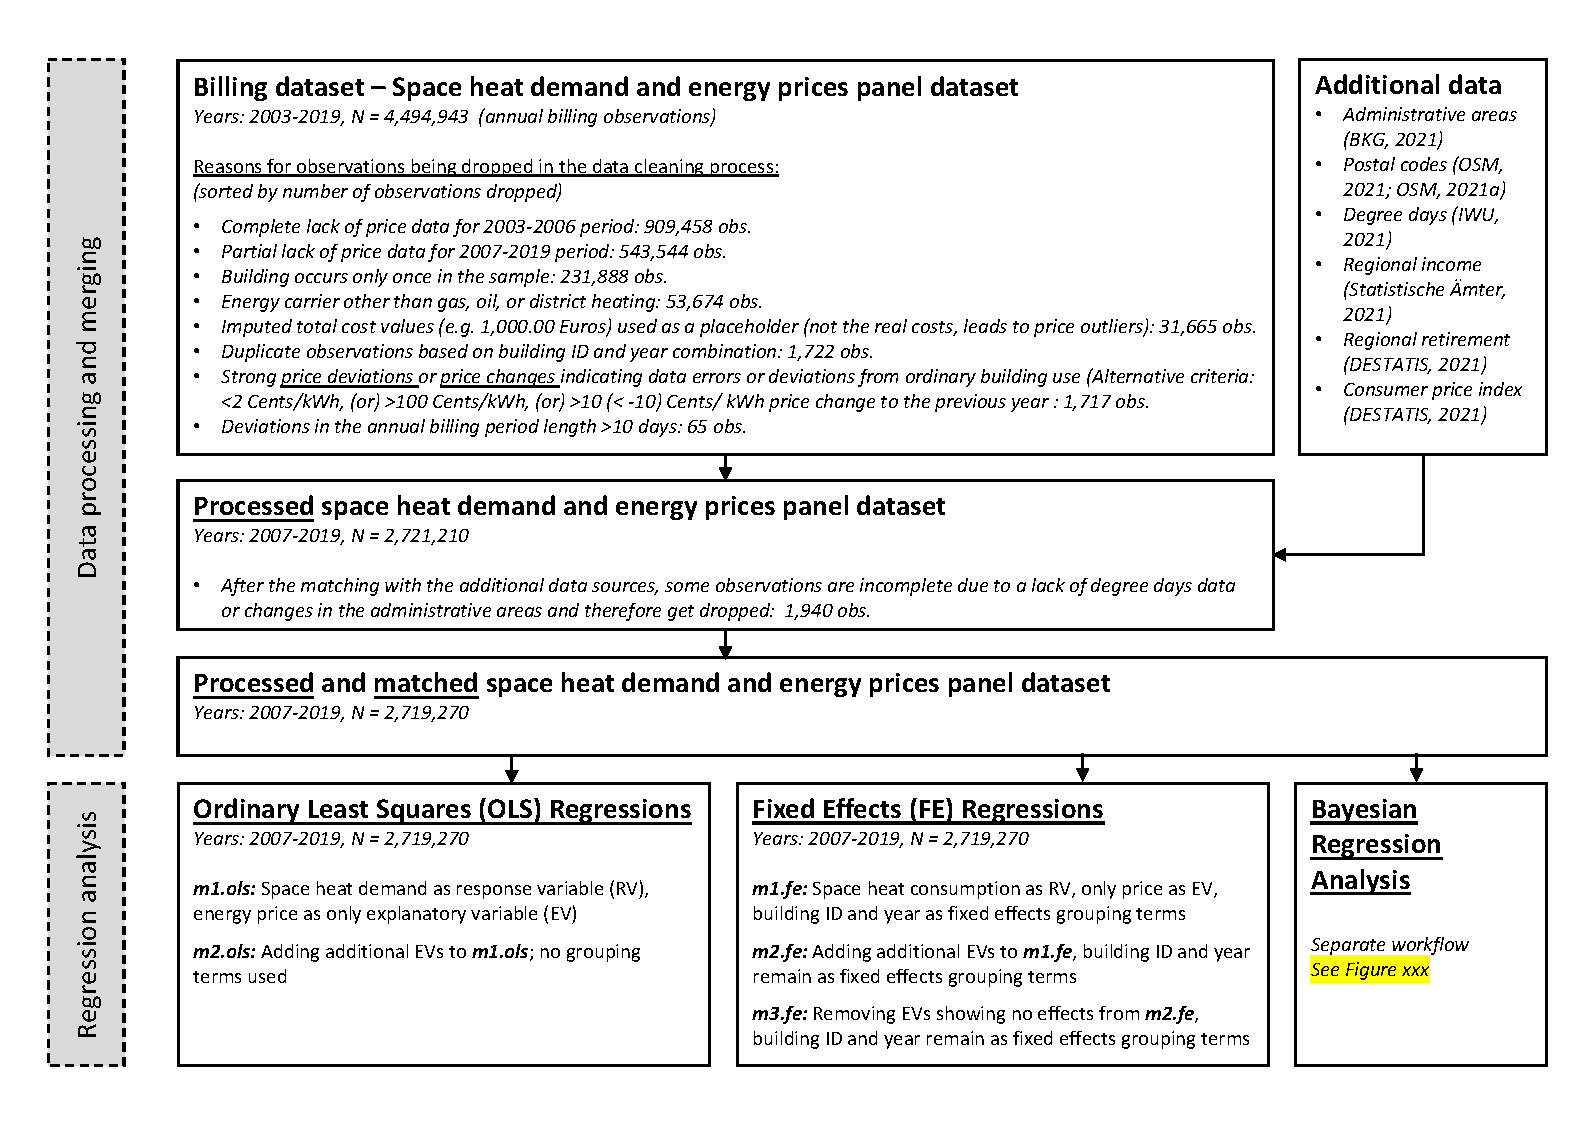
\includegraphics[width=1.03\linewidth]{figure/workflow_diagramm_1} 

}

\caption{Workflow of data processing and full sample analysis}\label{fig:workflow1}
\end{figure}
Spatial and temporal distribution:

In Appendix \ref{fig:buildings-distribution} the spatial and temporal distribution of observations is shown on the district-level. On the temporal dimension, structurally fewer observations of around 40,000 are available in 2007 and 2008, as price data were first recorded in these years. In the decade between 2009 and 2019, a minimum of 201,856 and an average of 239,183 buildings are observed annually, with good spatial coverage. There are only a few districts where no buildings are observed within a year, and for most district-year combinations more than 10 and up to more than 10,000 buildings are observed.

\hypertarget{notizen-aus-anderen-publikationen}{%
\section{Notizen aus anderen Publikationen}\label{notizen-aus-anderen-publikationen}}

Since we model conditional demand only, the results should be considered as short-term elasticities. In contrast, medium- and long-term income elasticities tend to be higher. Households with increased income are likely to move into larger homes over the medium term, which would increase their heating expenditures as well (Nesbakken 1999). --\textgreater{} Short-run elasticities as a lower bar estimate that produces a conservative estimate.

Csereklyei (2020):
It is widely anticipated that responses in electricity consumption to changes in prices will be rather slow, as it takes time for energy-using durable stock to change (Miller and Alberini, 2016). Thus, short-run or annual price elasticity estimates are expected to be rather inelastic, while one anticipates significantly larger long-run estimates.

Miller and Alberini (2016) furthermore report that the use of IV estimates can change the reported elasticities by up to 80\%.

All from Labanderira et al.

discrete decision to purchase durable goods that consume energy and the decision to consume energy is rarely considered.
renovations may disturbe the picture the panel data provides

On the other hand, most empirical studies in this area have used single-equation econometric models that require separability re- strictions. This is a severe disadvantage as it is not possible to estimate cross-price effects between different energy products or consider the effects of non-energy products on the price elasticity of energy goods.

Sample period. It is widely accepted that the economic cycle has a strong influence on energy consumption due to income and (indirect cycle-related) price effects. In the case of economic crises, for example, a depression of energy prices may occur; reduced dis- posable income may lead agents to reduce consumption through improvements in energy efficiency, adjustments to other types of consumption or changes towards other more inexpensive energy goods.

From Aufhammer wegen IV approach:
We instrument the utilities' consumer-facing prices with the weekly average spot price of natural gas at a major natural gas distribution hub in Louisiana (the Henry Hub). This instrument is valid, as we know the formula of how utilities pass-through the price (providing a strong first stage), and the price is determined prior to within-bill consumption (strengthening the exclusion restriction).

No change in the energy taxation (Energiesteuergesetz) in the observed period; letzte Neufassung aus 2006 mit Effekten für 2007

Miller Alberini (2016):
We also find that aggregating our data can result in both higher and lower price elasticity estimates, depending on the dataset used, and that controlling for unit-level fixed effects with panel data generally results in more inelastic demand functions. Addressing the endogeneity of price and/or measurement error in price with instrumental variables has a small but noticeable effect on the price elasticities. Finally, controlling for housing characteristics and capital stock produces a lower price elasticity.

\hypertarget{results}{%
\chapter{Results}\label{results}}

\hypertarget{descriptives}{%
\section{Descriptive statistics}\label{descriptives}}
\begin{figure}

{\centering 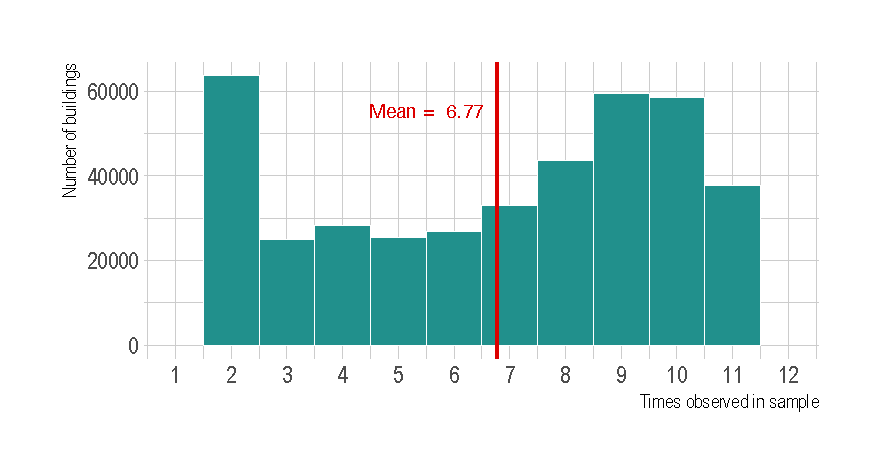
\includegraphics[width=0.65\linewidth]{figure/occurance_buildings} 

}

\end{figure}
\begin{table}[]
\centering
\caption{Summary statistics}
\label{tab:summarytable}
\begin{tabular}{@{}llc@{}}
\toprule
\textbf{Variable}             & \textbf{Unit}            & \textbf{Median (IQR)}   \\ \midrule
Space heat consumption, eff.  & {[}kWh/sqm.{]}           & 113 (86, 145)           \\
Energy price, real            & {[}Cents/kWh{]}          & 6.49 (5.77, 7.69)       \\
                              &                          &                         \\
Degree days                   &                          & 3,446 (3,214, 3,733)    \\
Building heating surface      & {[}sqm{]}                & 404 (260, 707)          \\
Building housing units        &                          & 6 (3, 10)               \\
District household income     & {[}€/a{]}                & 20,695 (18,786, 22,568) \\
District retirement share     & {[}\%{]}                 & 0.207 (0.193, 0.220)    \\
District population density   & {[}inhabitants/sq. km{]} & 572 (217, 1,960)        \\
                              &                          &                         \\
\textit{Energy carrier group} & {\ul \textit{}}          &                         \\
Gas                           &                          & 1,647,563 (61\%)        \\
Oil                           &                          & 802,451 (30\%)          \\
District heating              &                          & 268,232 (9.9\%)         \\ \midrule
\textit{(N = 2,718,246; No missings)}  &                          & \multicolumn{1}{l}{}   
\end{tabular}
\end{table}
\begin{figure}

{\centering 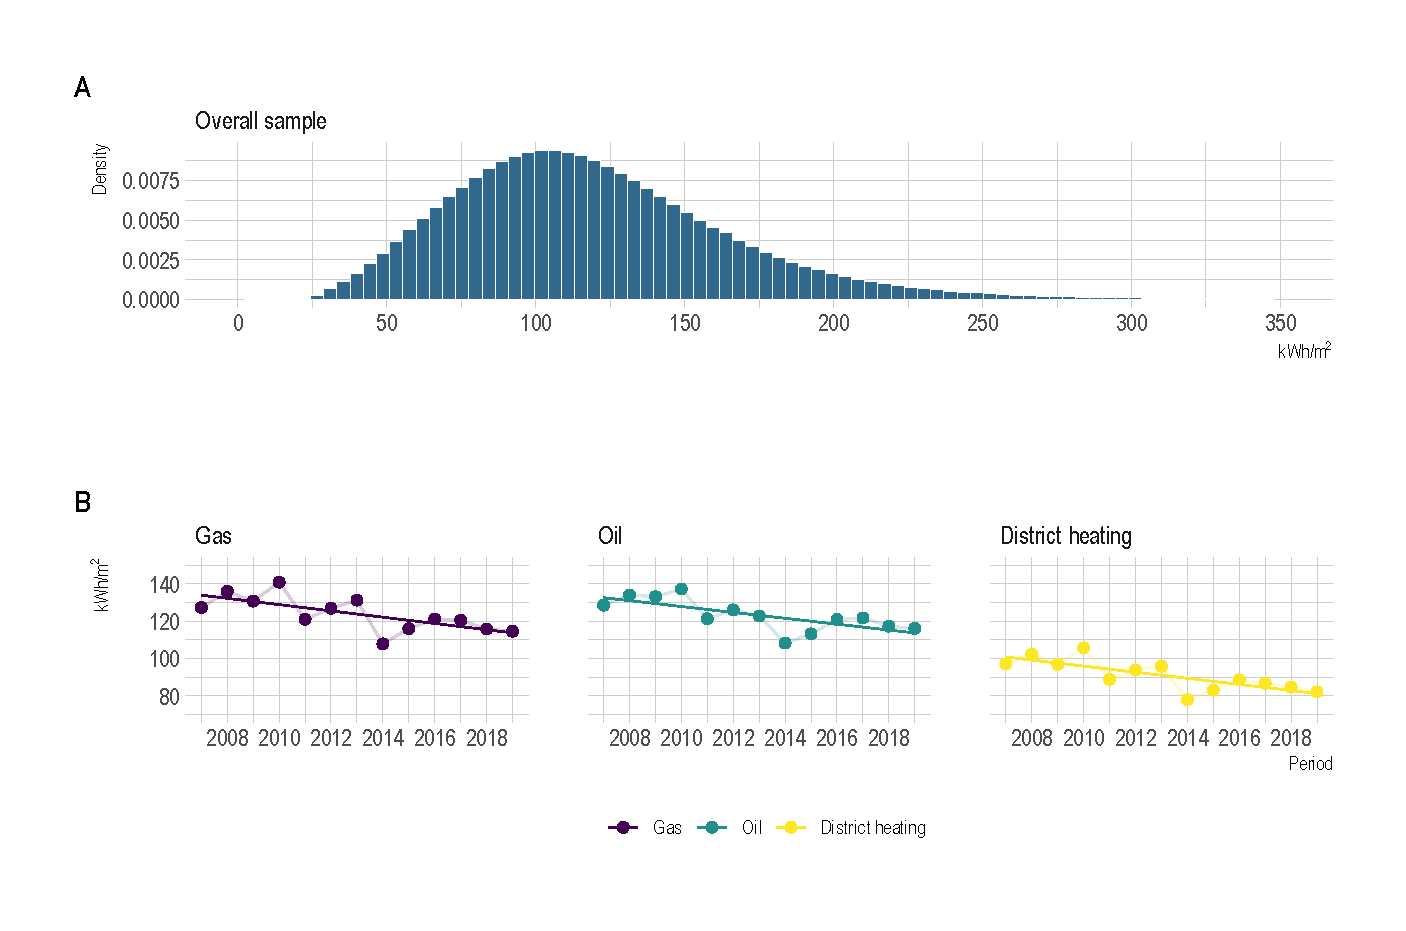
\includegraphics[width=1\linewidth]{figure/demand_descriptive} 

}

\caption{Distribution of energy demand}\label{fig:demand-descriptive-graph}
\end{figure}
\begin{figure}

{\centering 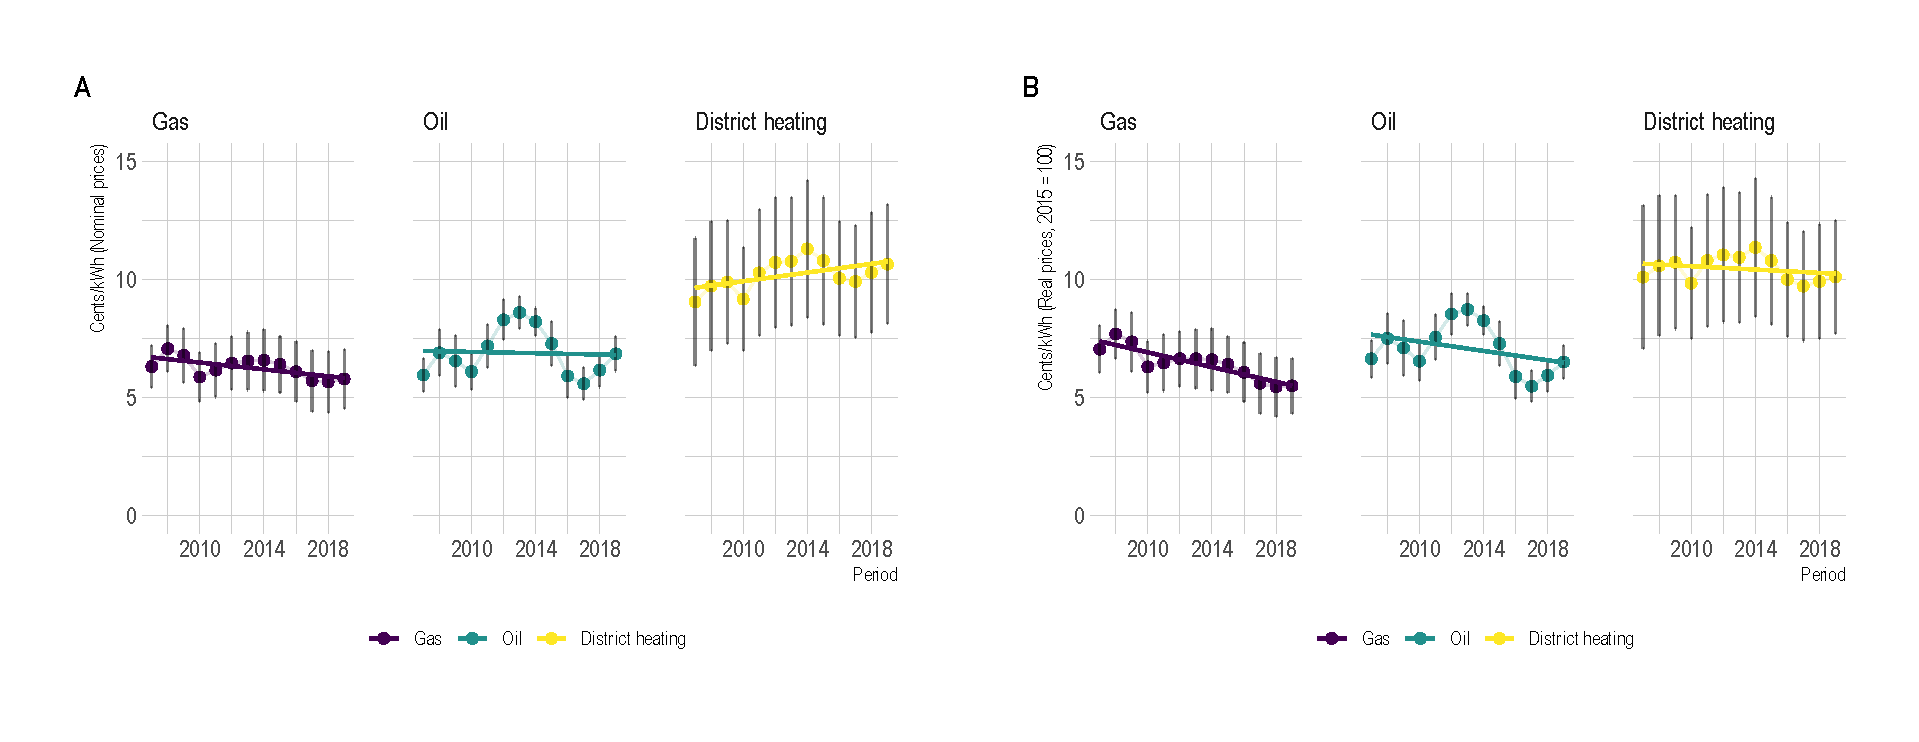
\includegraphics[width=1\linewidth]{figure/prices_descriptive} 

}

\caption{Distribution of nominal and real energy prices}\label{fig:price-descriptive-graph}
\end{figure}
\hypertarget{full_results}{%
\section{Full sample analysis}\label{full_results}}
\begin{table}[]
\centering
\caption{Regression table for full sample analysis}
\label{tab:reg-table-full-sample}
\resizebox{\textwidth}{!}{%
\begin{tabular}{llrrrrrr}
\cline{3-8}
 &  & \multicolumn{6}{c}{Response variable in all model specifications: Ln of space heat demand} \\
 &  & \multicolumn{2}{c}{OLS regression} & \multicolumn{1}{c}{} & \multicolumn{3}{c}{Fixed Effects (FE) regression} \\
\multicolumn{1}{c}{} & \multicolumn{1}{c}{} & \multicolumn{1}{c}{(1)} & \multicolumn{1}{c}{(2)} & \multicolumn{1}{c}{} & \multicolumn{1}{c}{(3)} & \multicolumn{1}{c}{(4)} & \multicolumn{1}{c}{(5)} \\ \cline{1-1} \cline{3-4} \cline{6-8} 
(Intercept) &  & 5.399 *** & 3.593 *** &  &  &  &  \\
 &  & (0.002) & (0.028) &  &  &  &  \\
\begin{tabular}[c]{@{}l@{}}Ln of\\ energy price\end{tabular} &  & -0.365 *** & -0.365 *** &  & -0.251 *** & -0.243 *** & -0.243 *** \\
 &  & (0.001) & (0.001) &  & (0.001) & (0.001) & (0.001) \\
\begin{tabular}[c]{@{}l@{}}Ln of\\ degree days\end{tabular} &  &  & 0.626 *** &  &  & 0.779 *** & 0.779 *** \\
 &  &  & (0.002) &  &  & (0.003) & (0.003) \\
\begin{tabular}[c]{@{}l@{}}Ln of\\ heating surface\end{tabular} &  &  & -0.133 *** &  &  & -0.405 *** & -0.405 *** \\
 &  &  & (0.000) &  &  & (0.003) & (0.003) \\
\begin{tabular}[c]{@{}l@{}}Energy carrier:\\ Oil\end{tabular} &  &  & 0.031 *** &  &  & 0.097 *** & 0.097 *** \\
 &  &  & (0.001) &  &  & (0.002) & (0.002) \\
\begin{tabular}[c]{@{}l@{}}Energy carrier:\\ District heating\end{tabular} &  &  & -0.061 *** &  &  & -0.020 *** & -0.020 *** \\
 &  &  & (0.001) &  &  & (0.002) & (0.002) \\
\begin{tabular}[c]{@{}l@{}}Ln of\\ district income\end{tabular} &  &  & -0.277 *** &  &  & 0.022 ** & 0.022 ** \\
 &  &  & (0.002) &  &  & (0.008) & (0.008) \\
\begin{tabular}[c]{@{}l@{}}Ln of district\\ population density\end{tabular} &  &  & 0.043 *** &  &  & 0,000 &  \\
 &  &  & (0.000) &  &  & (0.005) &  \\
\begin{tabular}[c]{@{}l@{}}Ln of\\ retirement share\end{tabular} &  &  & -0.084 *** &  &  & 0.435 *** & 0.435 *** \\
 &  &  & (0.010) &  &  & (0.030) & (0.030) \\ \cline{1-1} \cline{3-4} \cline{6-8} 
N &  & 2718246 & 2718246 &  & 2718246 & 2718246 & 2718246 \\
R2 &  & 0,049 & 0,156 &  & 0,822 & 0,829 & 0,829 \\
logLik &  & -1322263,852 & -1159565,133 &  &  &  &  \\
AIC &  & 2644533,703 & 2319150,267 &  &  &  &  \\ \cline{1-1} \cline{3-4} \cline{6-8} 
\multicolumn{8}{l}{*** p \textless 0.001;  ** p \textless 0.01;  * p \textless 0.05.}
\end{tabular}%
}
\end{table}
Notes (copied from other papers):

-Accounting for unobserved heterogeneity reduces the elasticities by 15\% to 32\% relative to a model that does not include any effects at all, where the own price elasticity of electricity demand is −1.).

\hypertarget{full_results}{%
\section{Subsample analysis}\label{full_results}}
\begin{figure}

{\centering 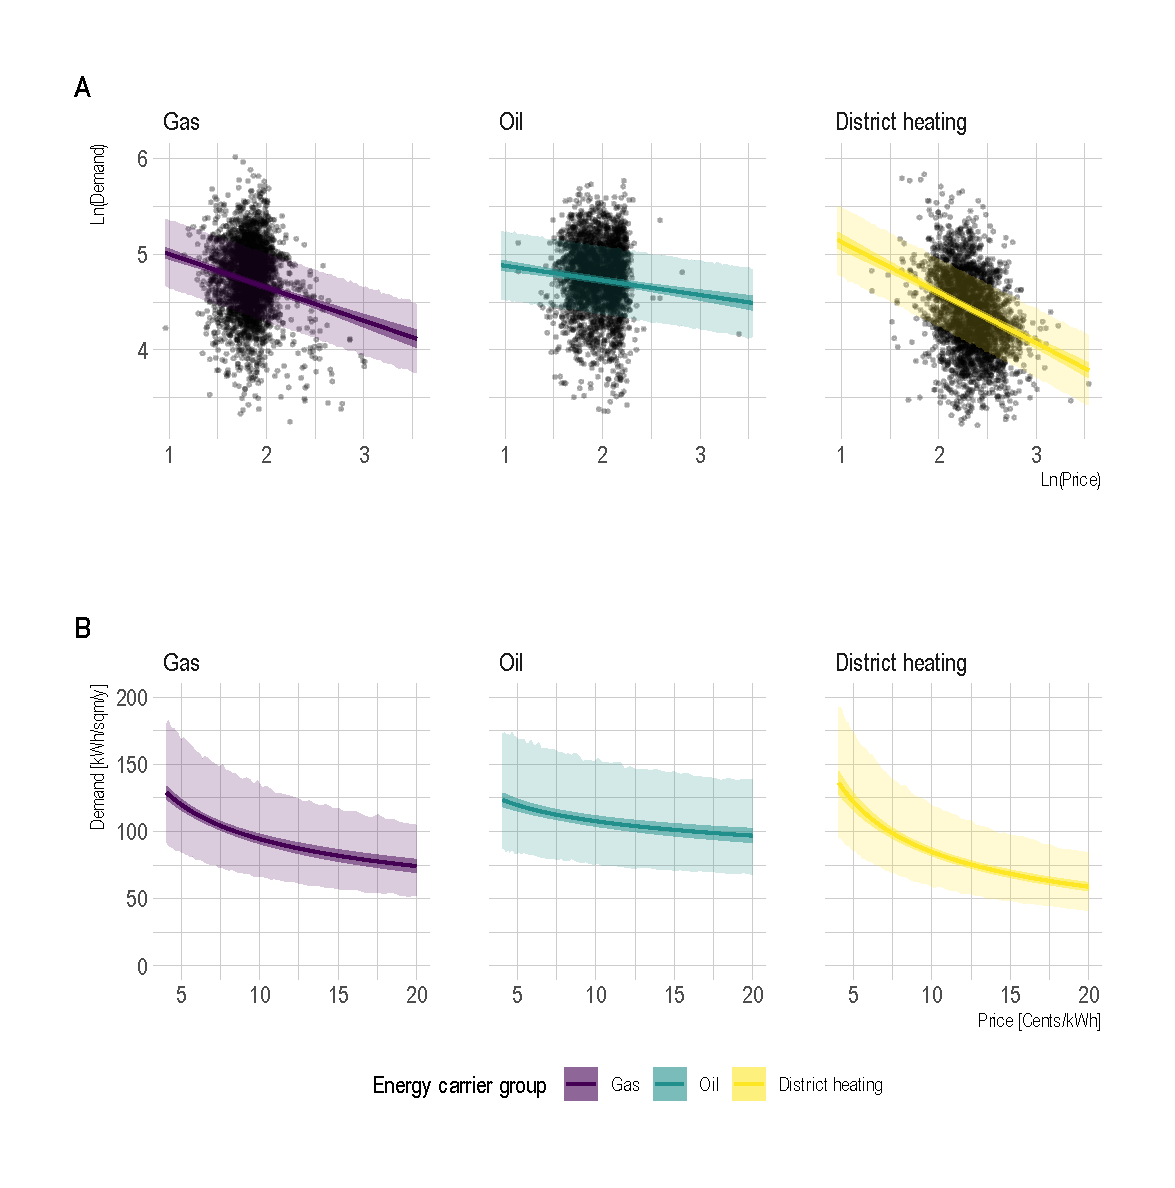
\includegraphics[width=1\linewidth]{figure/elasticity_predictions_subsample} 

}

\caption{Predicted price elasticities of demand by energy carrier}\label{fig:elasticity-predictions-subsample-graph}
\end{figure}
\hypertarget{discussion}{%
\chapter{Discussion}\label{discussion}}

NOTES - Energy taxation and climate change:
- Fuel consumption demand is determined by demand functions that depend primarily on income and prices
- Those who disfavor fuel taxes often claim they are strongly regressive. Earlier studies have shown that this depends on the country studied and on the details of the methods used, for instance if lifetime or temporary income is used, if substitution or other reactions are allowed for in the analysis. There is a tendency to progressivity in low income countries but regressivity in high income countries.
- Indirect channel of long-term price change and anticipation of those changes leading to investments in low-carbon UBA: Remediation measures drawn by lot through the BEHG are partly subsidized through the BEG or the tax incentive and are accounted for there (CO2 price as door opener for subsidy)

\hypertarget{discussion-of-elasticity-results}{%
\section{Discussion of elasticity results}\label{discussion-of-elasticity-results}}

\hypertarget{the-role-of-energy-prices-and-interaction-with-complementary-measures}{%
\section{The role of energy prices and interaction with complementary measures}\label{the-role-of-energy-prices-and-interaction-with-complementary-measures}}
\begin{itemize}
\item
  For district heating larger share of costs are fixed; may drive the effect of larger price elasticities as data does not differentiate between fixed and variable cost components and with lower energy demand the per-unit cost rate increses due to the larger
\item
  Prices not the only option for action, potential overestimation of price relevance
\item
  Warmmietenmodell (Now only the renters are effected which will mainly trigger short-term price reactions; for decarbonisation need to tap the long-term channel; Lessors must be incentivized to initialize efficiency measures; one option: split prices but then long-term price signal is still partly muted; Warmmietmodell as an alternative where both parties renters and lessors have full economic incentive of pricing measures)
\end{itemize}
\hypertarget{conclusion}{%
\chapter{Conclusion}\label{conclusion}}

\eqref{eq:ep}

\appendix

\hypertarget{additional-materials}{%
\chapter{Additional materials}\label{additional-materials}}

\singlespacing
\newpage
\begin{figure}

{\centering 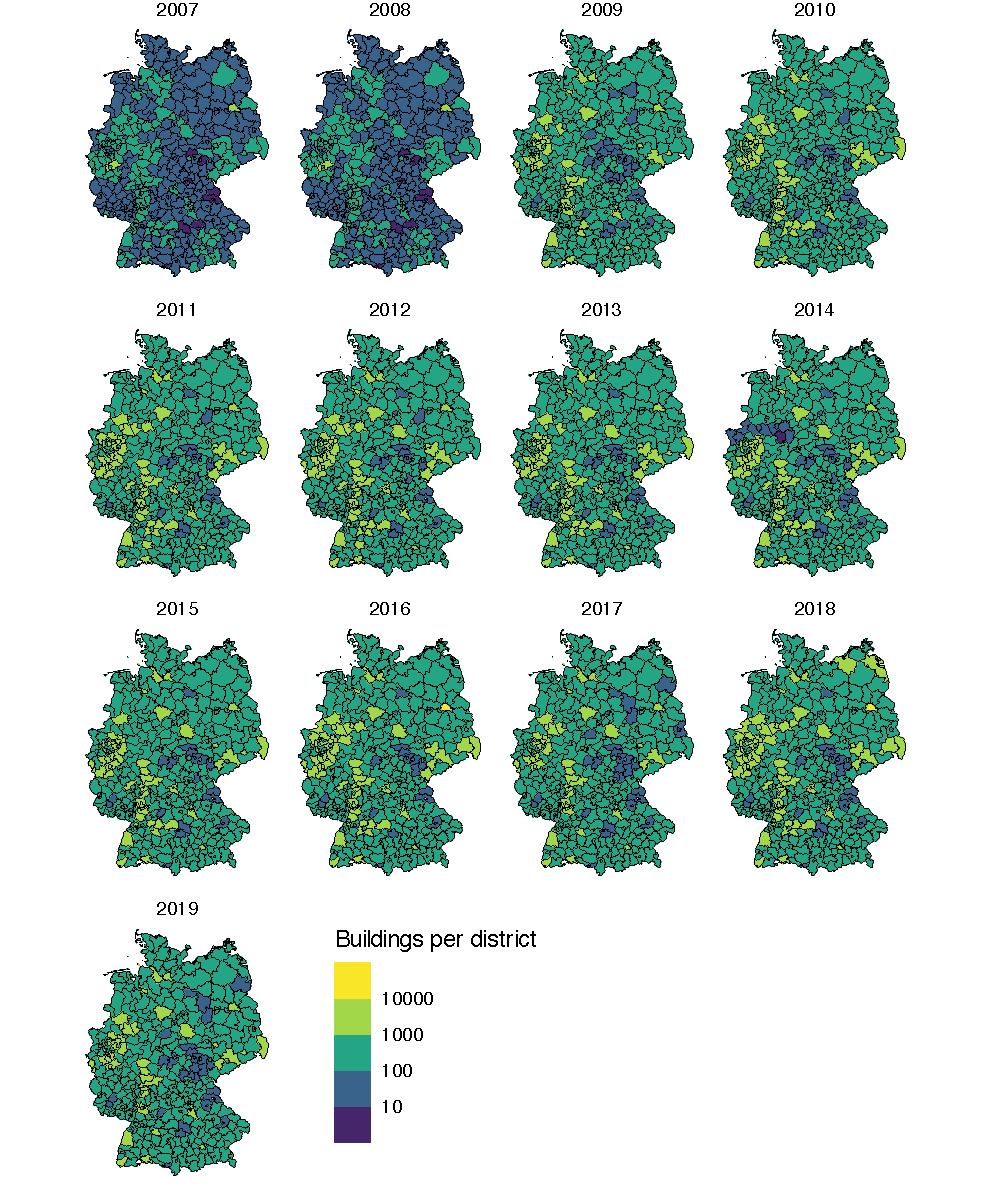
\includegraphics[width=0.77\linewidth]{figure/buildings_distribution} 

}

\caption{Spatial and temporal coverage by the buildings observed}\label{fig:buildings-distribution}
\end{figure}
\noindent
Figure \ref{fig:buildings-distribution} shows the spatial and temporal distribution of observations at building-level in the main sample. The maps show that the spatial coverage is good. There are very few districts without observations (transparent) and only a few districts with less than 10 observed buildings per year (dark blue). For most district-year combinations, more than 100 buildings are observed. In some large cities and metropolitan areas, numbers of more than 10,000 buildings are reached. Fewer observations are available for 2007 (43,696 observations) and 2008 (43,536 observations), as price data were included for the first time in these years. For the decade between 2009 and 2019, an annual minimum of 201,856 and an average of 239,183 buildings are observed. Note the use of the logarithmic scale in the maps.

\newpage
\begin{figure}

{\centering 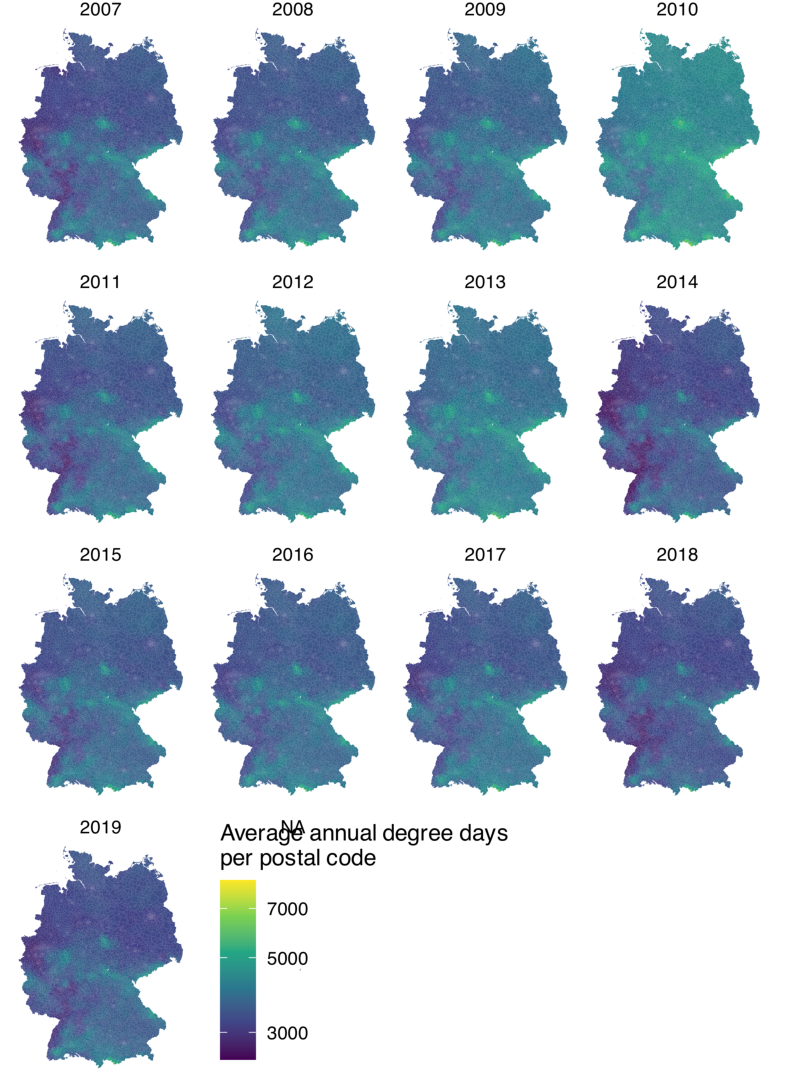
\includegraphics[width=0.77\linewidth]{figure/distribution_degree_days} 

}

\caption{Spatial and temporal variation in degree days}\label{fig:degree-days-distribution}
\end{figure}
\noindent
Figure \ref{fig:degree-days-distribution} show the spatial and temporal variation of climatic conditions measured in degree days. Degree days are extracted from \protect\hyperlink{ref-iwu21}{IWU} (\protect\hyperlink{ref-iwu21}{2021}). The spatial resolution used is the postcode level as the level with the highest granularity, which is also used in the regressions. Higher annual degree day numbers are associated with lower outdoor temperatures and vice versa. The maps show variations between the observed annual periods. While 2010 in particular, but also 2012 and 2013 are cooler years than the sample average, 2014, 2018 and 2019, on the other hand, were considerably warmer.

\newpage
\begin{figure}

{\centering 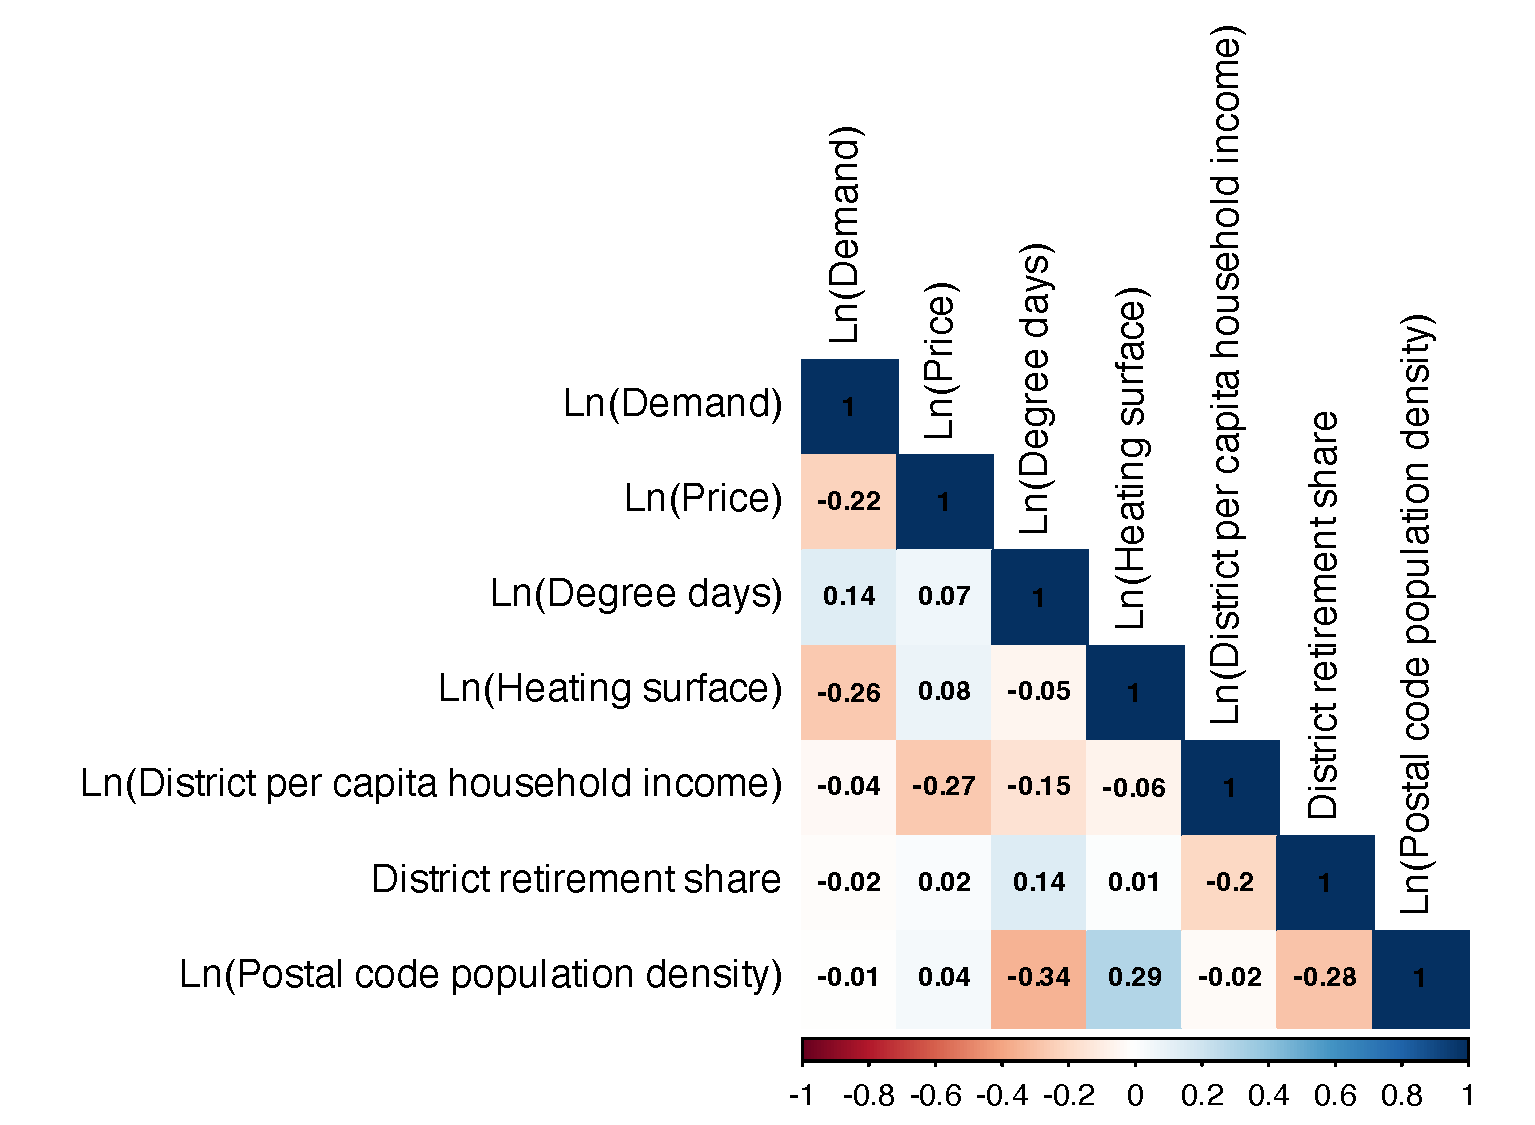
\includegraphics[width=0.9\linewidth]{figure/correlation_matrix} 

}

\caption{Pearson’s correlation matrix}\label{fig:correlation-plot}
\end{figure}
\noindent
The values in Figure \ref{fig:correlation-plot} represent Pearson's correlation coefficients. Values closer to 1 indicate a stronger positive relationship, values closer to -1 indicate a stronger negative relationship. Values close to zero indicate no relationship. None of the correlations observed between the variables exceed moderate values, ruling out possible multicollinearity issues. Energy price is negatively correlated with energy demand, indicating that the expected negative effect of price on demand indeed exists. Note that tall variables are ln-transformed.

\newpage
\begin{table}[]
\centering
\caption{Comparison between full sample and sub-sample}
\label{tab:sample-comparison}
\resizebox{\textwidth}{!}{%
\begin{tabular}{@{}lllll@{}}
\toprule
Variable                                                                                       & Energy carrier group & \begin{tabular}[c]{@{}l@{}}Full sample\\ (N = 2.719.270)\end{tabular} & \begin{tabular}[c]{@{}l@{}}Sub-sample\\ (N = 4.410)\end{tabular} & Difference {[}\%{]}       \\ \midrule
\multirow{3}{*}{\begin{tabular}[c]{@{}l@{}}Energy demand\\ {[}kWh/m2{]}\end{tabular}}          & Gas                  & 122.5 {[}56.4; 209.33{]}                                              & 121.39 {[}55.4; 211.32{]}                                        & -0.91 {[}-1.81; 0.94{]}   \\
                                                                                               & Oil                  & 122.36 {[}58.67; 204{]}                                               & 116.97 {[}53.57; 198.17{]}                                       & -4.61 {[}-9.52; -2.94{]}  \\
                                                                                               & District heating     & 89.38 {[}43.23; 156.88{]}                                             & 83.98 {[}41.92; 141.01{]}                                        & -6.43 {[}-3.12; -11.25{]} \\
\multicolumn{5}{l}{} \\                                                                                                 
\multirow{3}{*}{\begin{tabular}[c]{@{}l@{}}Energy price, real \\ {[}Cents/kWh{]}\end{tabular}}        & Gas                  & 6.28 {[}4.56; 8.14{]}                                                 & 6.22 {[}4.59; 8.04{]}                                            & -0.96 {[}0.65; -1.24{]}   \\
                                                                                               & Oil                  & 7.14 {[}5.1; 9.18{]}                                                  & 7.21 {[}5.2; 9.23{]}                                             & 0.97 {[}1.92; 0.54{]}     \\
                                                                                               & District heating     & 10.45 {[}6.86; 15.07{]}                                               & 10.76 {[}7.17; 16.15{]}                                          & 2.88 {[}4.32; 6.69{]}     \\
\multicolumn{5}{l}{} \\   
\multirow{3}{*}{Degree days}                                                                   & Gas                  & 3467.6 {[}2921.14; 4180.42{]}                                         & 3461.14 {[}2914.56; 4180.4{]}                                    & -0.19 {[}-0.23; 0{]}      \\
                                                                                               & Oil                  & 3568.13 {[}2971.7; 4269.19{]}                                         & 3582.48 {[}2946.19; 4318.42{]}                                   & 0.4 {[}-0.87; 1.14{]}     \\
                                                                                               & District heating     & 3441.1 {[}2924.64; 4137.61{]}                                         & 3447.97 {[}2948.92; 4180.11{]}                                   & 0.2 {[}0.82; 1.02{]}      \\
\multicolumn{5}{l}{} \\   
\multirow{3}{*}{\begin{tabular}[c]{@{}l@{}}Building heating \\ surface {[}sqm{]}\end{tabular}} & Gas                  & 648.84 {[}163; 1849.4{]}                                              & 727.47 {[}168.04; 1817{]}                                        & 10.81 {[}3; -1.78{]}      \\
                                                                                               & Oil                  & 452.82 {[}160; 1195.6{]}                                              & 489.55 {[}167.1; 1362.8{]}                                       & 7.5 {[}4.25; 12.27{]}     \\
                                                                                               & District heating     & 1714.09 {[}255; 5030.18{]}                                            & 2034.55 {[}297.52; 6968.98{]}                                    & 15.75 {[}14.29; 27.82{]}  \\ \midrule
\multicolumn{5}{l}{\textit{*) Mean {[}90\% CI{]}}}                                                                                                                                                                                                                                          
\end{tabular}%
}
\end{table}
\noindent
Table \ref{tab:sample-comparison} compares the total sample and the sub-sample with respect to key variables. It contains the mean values for the two samples and the lower and upper limits of a 90\% interval divided by the energy carrier. It also gives the relative difference between the total sample and the sub-sample in percent. The statistics show that in the sub-sample with the available epc information, the buildings are on average 7.5 \% to 15.8 \% larger, depending on the energy carrier. This deviation is presumably due to the fact that larger buildings are more often managed by larger property managers who decide to systematically exchange their information with ista and also obtain their energy performance certificates through this standardised channel. The larger building heating area is likely also the reason for the deviations between the total sample and the sub-sample in energy demand for oil (-4.6\%) and district heating (-6.4\%). However, the deviations are within reasonable limits. Energy price and degree days from both samples are in good agreement.

\newpage
\begin{figure}

{\centering 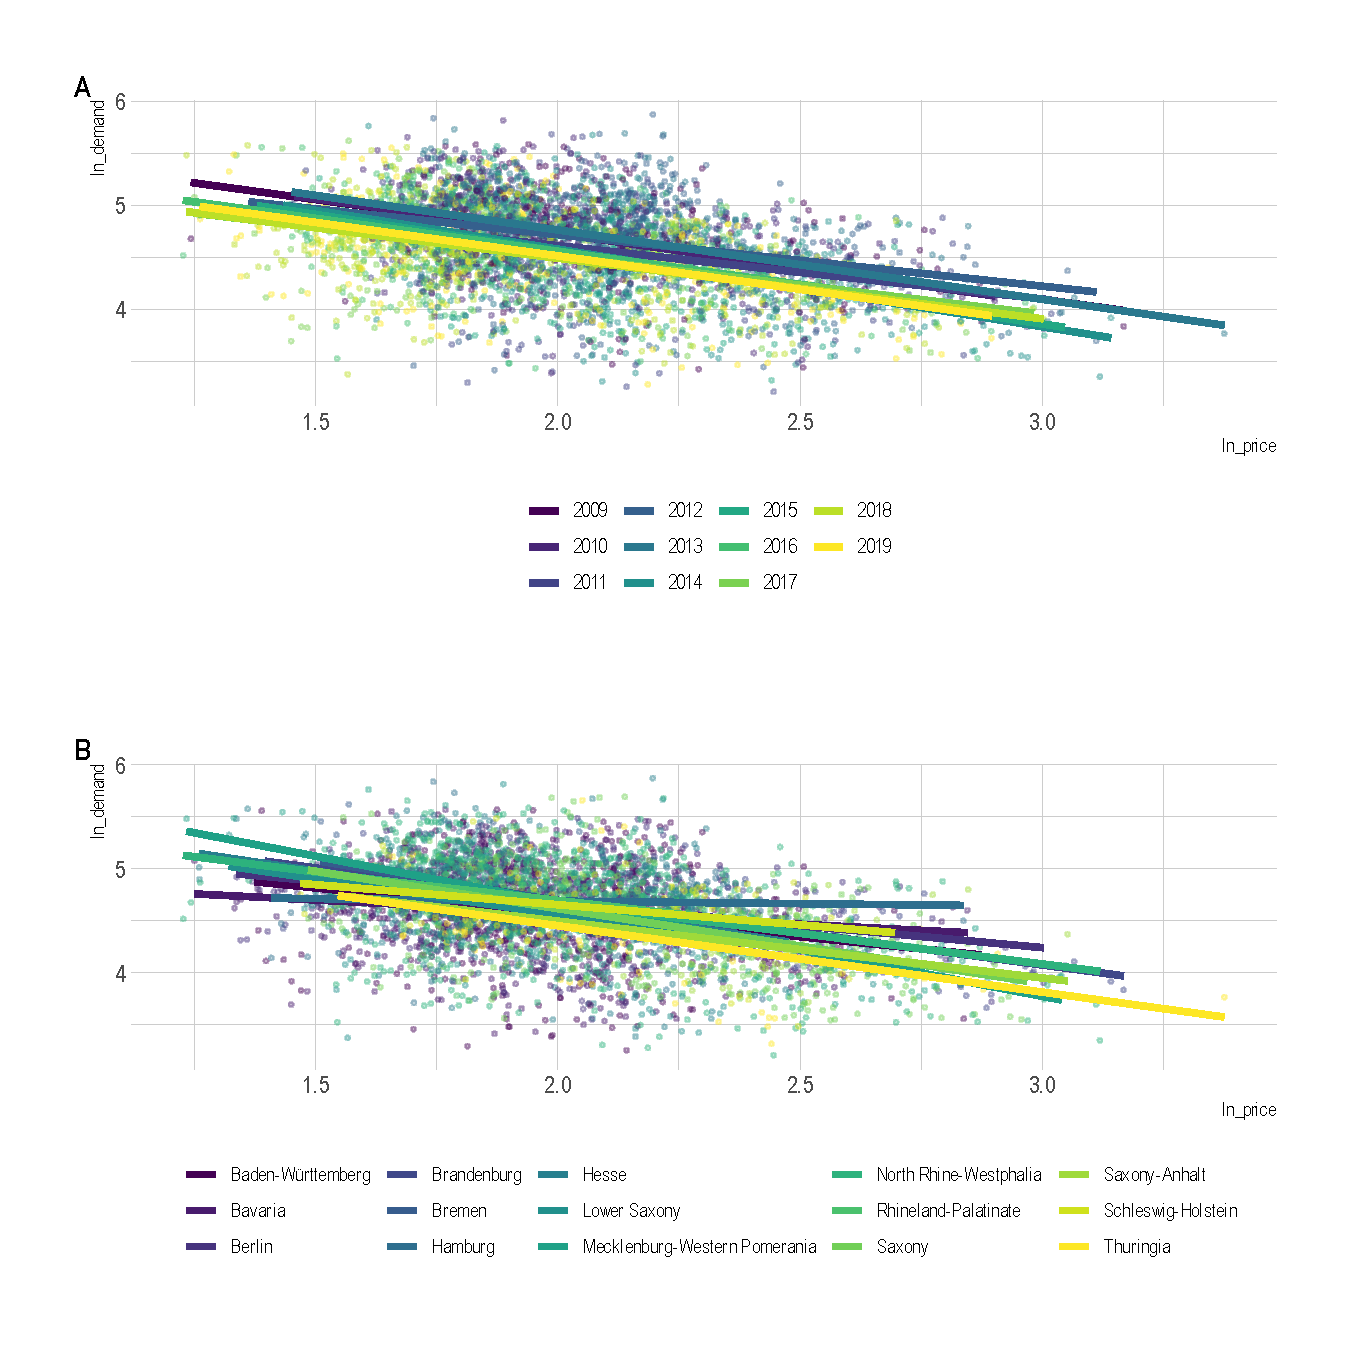
\includegraphics[width=1\linewidth]{figure/year_state_heterogeneity_plot} 

}

\caption{Investigation of heterogeneity for years and federal states}\label{fig:heterogeneity-year-state-plot}
\end{figure}
\noindent
Figure \ref{fig:heterogeneity-year-state-plot} presents a visual examination of the heterogeneity of price elasticity between years (Panel A) and federal states (Panel B). For this purpose, the observations in the sub-sample are grouped by year/federal state and presented in a scatter plot. The lines in the diagrams reflect simple linear models for the years/federal states as groups. Between years, all lines are almost parallel, indicating that there is no relevant difference in price elasticity between years. For the federal states, the lines scatter a little. At the same time, however, no strong pattern can be discerned through clusters such as differences between formerly eastern and western federal states or through other regional clusters.

\newpage
\begin{figure}

{\centering 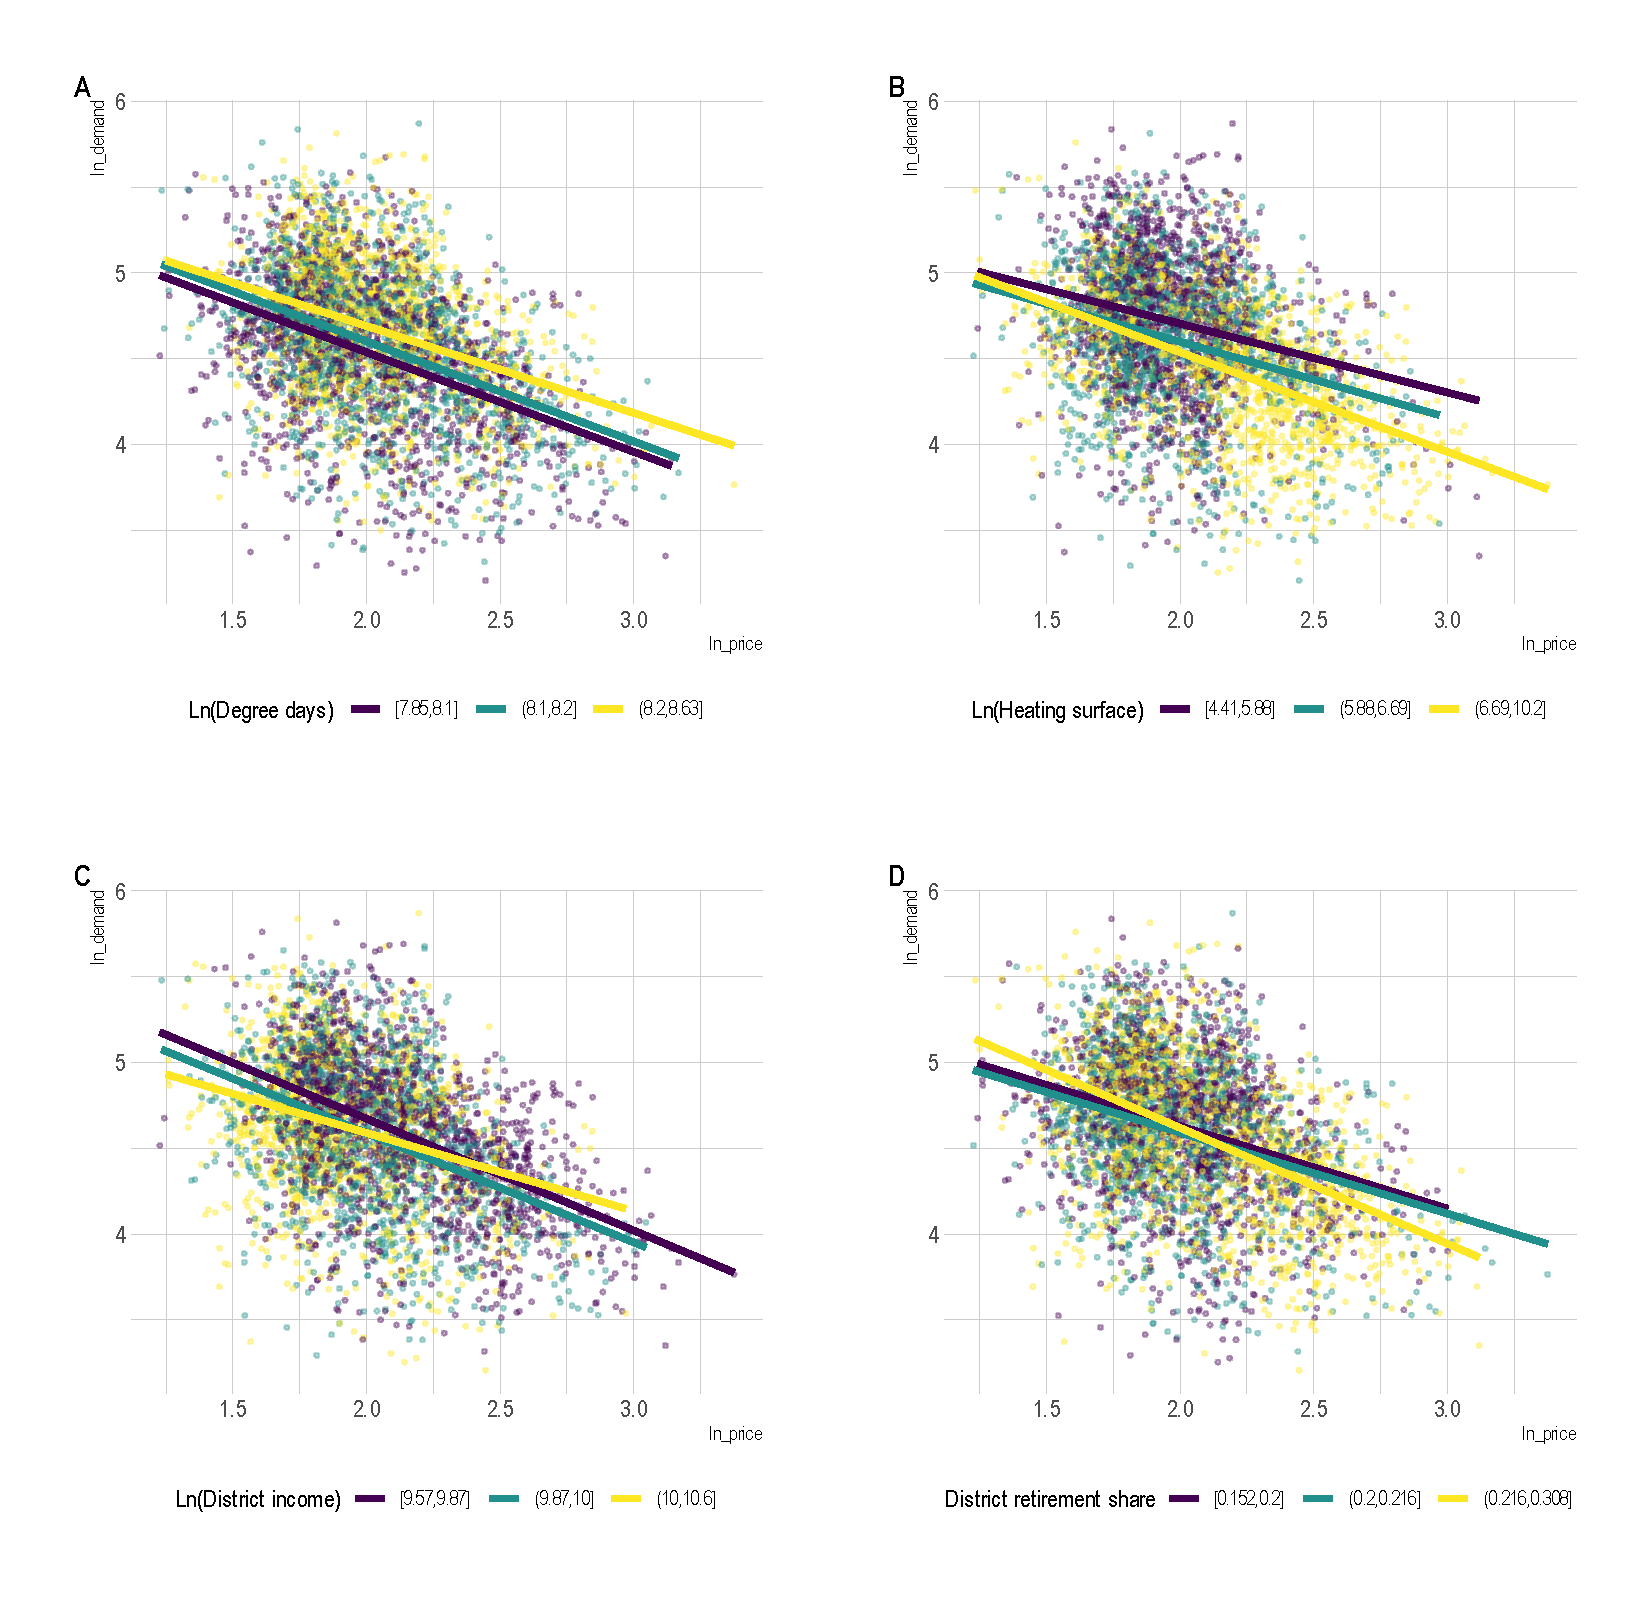
\includegraphics[width=0.95\linewidth]{figure/other_vars_heterogeneity_plot} 

}

\caption{Investigation of heterogeneity for degree days, heating surface, district income, and district retirement share}\label{fig:heterogeneity-other-vars-plot}
\end{figure}
\noindent
Figure \ref{fig:heterogeneity-other-vars-plot} presents a visual examination of the heterogeneity of price elasticity for the four variables degree days (Panel A), building heating surface (Panel B), average district income (Panel C), and district retirement share (Panel D). Since all four variables represent continuous variables, observations in the sub-sample are ln-transformed, grouped into three equally sized groups,\footnote{E.g., one third of observations with lowest number of degree days (between 7.85 and 8.1), one third of observations medium number of degree days (between 8.1 and 8.2), and one third of observations highest number of degree days (between 8.2 and 8.63).} and presented in a scatter plot. The lines in the diagrams reflect simple linear models for the respective three groups of equal size. For degree days, the lines are almost parallel and show no difference in price elasticity. For the other three variables, a slight dispersion of the grouped lines can be observed. But again, there are no pronounced differences that would prompt a more detailed investigation.

\newpage

\textbf{Delete later}

\begingroup\fontsize{10}{12}\selectfont
\begin{longtable}[t]{lr}
\caption{\label{tab:tabletest}Number of flight connections per destination}\\
\toprule
Destination & Number of connections\\
\midrule
\endfirsthead
\caption[]{\label{tab:tabletest}Number of flight connections per destination \textit{(continued)}}\\
\toprule
Destination & Number of connections\\
\midrule
\endhead

\endfoot
\bottomrule
\multicolumn{2}{l}{\rule{0pt}{1em}\textsuperscript{1} This table was created based on the flights dataset.}\\
\multicolumn{2}{l}{\rule{0pt}{1em}\textsuperscript{2} Source: R Packages.}\\
\endlastfoot
Albuquerque International Sunport & 30\\
Bob Hope & 261\\
Boise Air Terminal & 29\\
Charlotte Douglas Intl & 45\\
Chicago Midway Intl & 104\\
\addlinespace
Chicago Ohare Intl & 524\\
Dallas Fort Worth Intl & 441\\
Denver Intl & 905\\
Detroit Metro Wayne Co & 55\\
General Edward Lawrence Logan Intl & 70\\
\addlinespace
George Bush Intercontinental & 228\\
Hartsfield Jackson Atlanta Intl & 410\\
Honolulu Intl & 180\\
John F Kennedy Intl & 137\\
John Wayne Arpt Orange Co & 247\\
\addlinespace
Kahului & 171\\
Kansas City Intl & 89\\
Klamath Falls Airport & 82\\
Kona Intl At Keahole & 90\\
Lihue & 52\\
\addlinespace
Long Beach & 263\\
Los Angeles Intl & 912\\
Mahlon Sweet Fld & 189\\
Mc Carran Intl & 564\\
Metropolitan Oakland Intl & 451\\
\addlinespace
Minneapolis St Paul Intl & 270\\
Newark Liberty Intl & 91\\
Norman Y Mineta San Jose Intl & 574\\
Ontario Intl & 196\\
Palm Springs Intl & 105\\
\addlinespace
Phoenix Sky Harbor Intl & 888\\
Reno Tahoe Intl & 94\\
Roberts Fld & 252\\
Ronald Reagan Washington Natl & 87\\
Sacramento Intl & 404\\
\addlinespace
Salt Lake City Intl & 538\\
San Diego Intl & 265\\
San Francisco Intl & 1265\\
Santa Barbara Muni & 89\\
Seattle Tacoma Intl & 569\\
\addlinespace
Ted Stevens Anchorage Intl & 254\\
Tucson Intl & 90\\
Washington Dulles Intl & 89\\*
\end{longtable}
\endgroup{}

\onehalfspacing

\hypertarget{declaration-of-authorship-eigenstuxe4ndigkeitserkluxe4rung}{%
\chapter*{Declaration of Authorship (Eigenständigkeitserklärung)}\label{declaration-of-authorship-eigenstuxe4ndigkeitserkluxe4rung}}
\addcontentsline{toc}{chapter}{Declaration of Authorship (Eigenständigkeitserklärung)}

Hiermit erkläre ich, dass ich die vorliegende Arbeit selbständig verfasst habe und sämtliche Quellen, einschließlich Internetquellen, die unverändert oder abgewandelt wiedergegeben werden, insbesondere Quellen für Texte, Grafiken, Tabellen und Bilder, als solche kenntlich gemacht habe.

Ich versichere, dass ich die vorliegende Abschlussarbeit noch nicht für andere Prüfungen eingereicht habe.

Mir ist bekannt, dass bei Verstößen gegen diese Grundsätze ein Verfahren wegen Täuschungsversuchs bzw. Täuschung gemäß der fachspezifischen Prüfungsordnung und/oder der Fächerübergreifenden Satzung zur Regelung von Zulassung, Studium und Prüfung der Humboldt-Universität zu Berlin (ZSP-HU) eingeleitet wird.

\hfill\break
~

\hfill\break
~

\hfill\break
~
\begin{tabular}{m{6cm}m{2cm}m{6cm}}
Berlin, den 28.02.2022 &  &              \\ \cline{1-1} \cline{3-3} 
\textit{Ort, Datum}            &  & \textit{Unterschrift} \\
                       &  &              \\
                       &  &             
\end{tabular}
\backmatter

\hypertarget{references}{%
\chapter*{References}\label{references}}
\addcontentsline{toc}{chapter}{References}

\markboth{References}{References}

\noindent

\setlength{\parindent}{-0.20in}

\hypertarget{refs}{}
\begin{CSLReferences}{1}{0}
\leavevmode\vadjust pre{\hypertarget{ref-ageb21}{}}%
AGEB. (2021). \emph{Auswertungstabellen zur Energiebilanz 1990 bis 2020}. Berlin. Retrieved from \url{https://ag-energiebilanzen.de/daten-und-fakten/auswertungstabellen/}

\leavevmode\vadjust pre{\hypertarget{ref-alberini_etal11}{}}%
Alberini, A., Gans, W., \& Velez-Lopez, D. (2011). Residential consumption of gas and electricity in the U.S.: The role of prices and income. \emph{Energy Economics}, \emph{33}(5), 870--881. http://doi.org/\href{https://doi.org/10.1016/j.eneco.2011.01.015}{10.1016/j.eneco.2011.01.015}

\leavevmode\vadjust pre{\hypertarget{ref-aldy_etal10}{}}%
Aldy, J. E., Krupnick, A. J., Newell, R. G., Parry, I. W. H., \& Pizer, W. A. (2010). Designing Climate Mitigation Policy. \emph{Journal of Economic Literature}, \emph{48}(4), 903--934. http://doi.org/\href{https://doi.org/10.1257/jel.48.4.903}{10.1257/jel.48.4.903}

\leavevmode\vadjust pre{\hypertarget{ref-auffhammer_rubin18}{}}%
Auffhammer, M., \& Rubin, E. (2018). \emph{Natural Gas Price Elasticities and Optimal Cost Recovery Under Consumer Heterogeneity: Evidence from 300 million natural gas bills} (No. w24295) (p. w24295). Cambridge, MA: National Bureau of Economic Research. Retrieved from \url{http://www.nber.org/papers/w24295.pdf}

\leavevmode\vadjust pre{\hypertarget{ref-bmwi21}{}}%
BMWi. (2021). \emph{Gesamtausgabe der Energiedaten}. BMWi. Retrieved from \url{https://www.bmwi.de/Redaktion/DE/Binaer/Energiedaten/energiedaten-gesamt-xls.xlsx?__blob=publicationFile\&v=133}

\leavevmode\vadjust pre{\hypertarget{ref-burger_etal19}{}}%
Bürger, V., Hesse, T., Köhler, B., Palzer, A., \& Engelmann, P. (2019). German Energiewende---different visions for a (nearly) climate neutral building sector in 2050. \emph{Energy Efficiency}, \emph{12}(1), 73--87. http://doi.org/\href{https://doi.org/10.1007/s12053-018-9660-6}{10.1007/s12053-018-9660-6}

\leavevmode\vadjust pre{\hypertarget{ref-csereklyei20}{}}%
Csereklyei, Z. (2020). Price and income elasticities of residential and industrial electricity demand in the European Union. \emph{Energy Policy}, \emph{137}, 111079. http://doi.org/\href{https://doi.org/10.1016/j.enpol.2019.111079}{10.1016/j.enpol.2019.111079}

\leavevmode\vadjust pre{\hypertarget{ref-cutler41}{}}%
Cutler, H. A. (1941). The Elasticity of the Residential Demand for Electricity. \emph{The Journal of Land \& Public Utility Economics}, \emph{17}(2), 242--245. http://doi.org/\href{https://doi.org/10.2307/3158428}{10.2307/3158428}

\leavevmode\vadjust pre{\hypertarget{ref-destatis18}{}}%
DESTATIS. (2018). Fernwärmeversorgung 2017: Abgegebene Wärmemenge leicht gesunken. Retrieved January 19, 2022, from \url{https://www.destatis.de/DE/Presse/Pressemitteilungen/2018/11/PD18_434_434.html}

\leavevmode\vadjust pre{\hypertarget{ref-destatis21c}{}}%
DESTATIS. (2021a). Bevölkerung: Kreise, Stichtag, Altersgruppen (12411-0017) {[}Text{]}. Retrieved January 22, 2022, from \url{https://www-genesis.destatis.de/genesis/online?operation=previous\&levelindex=0\&step=0\&titel=Tabellenaufbau\&levelid=1642855066461\&acceptscookies=false\#abreadcrumb}

\leavevmode\vadjust pre{\hypertarget{ref-destatis21}{}}%
DESTATIS. (2021b, November 12). Verbraucherpreisindex: Deutschland, Jahre (61111-0001). Retrieved November 12, 2021, from \url{https://www-genesis.destatis.de/genesis//online?operation=table\&code=61111-0001\&bypass=true\&levelindex=1\&levelid=1636748679996\#abreadcrumb}

\leavevmode\vadjust pre{\hypertarget{ref-erk20}{}}%
ERK. (2020). \emph{Bericht zur Vorjahresschätzung der deutschen Treibhausgasemissionen für das Jahr 2020}. Retrieved from \url{https://expertenrat-klima.de/content/uploads/2021/04/210415_Bericht_Expertenrat_Klimafragen_2021-2.pdf}

\leavevmode\vadjust pre{\hypertarget{ref-europeancomission19}{}}%
European Comission. (2019). \emph{The European Green Deal} (No. COM(2019) 640 final). Brussels. Retrieved from \url{https://eur-lex.europa.eu/legal-content/EN/TXT/HTML/?uri=CELEX:52019DC0640\&from=EN}

\leavevmode\vadjust pre{\hypertarget{ref-gwartney76}{}}%
Gwartney, J. D. (1976). Demand and Consumer Choice. In \emph{Economics Private and Public Choice} (pp. 289--309). Elsevier. http://doi.org/\href{https://doi.org/10.1016/B978-0-12-311050-3.50021-8}{10.1016/B978-0-12-311050-3.50021-8}

\leavevmode\vadjust pre{\hypertarget{ref-halbig_namyslo14}{}}%
Halbig, G., \& Namyslo, J. (2014). Neue Witterungsbereinigung für Energieausweise auf der Basis des Referenzklimas Potsdam. \emph{EneV aktuell}, (4), 11--13.

\leavevmode\vadjust pre{\hypertarget{ref-hennes_etal21}{}}%
Hennes, O., Jeddi, S., Madlener, R., Schmitz, H., Wagner, J., Wolff, S., \& Zinke, J. (2021). Auswirkungen von CO2-Preisen auf den Gebäude‑, Verkehrs- und Energiesektor. \emph{Zeitschrift für Energiewirtschaft}, \emph{45}(2), 91--107. http://doi.org/\href{https://doi.org/10.1007/s12398-021-00305-0}{10.1007/s12398-021-00305-0}

\leavevmode\vadjust pre{\hypertarget{ref-hesse20}{}}%
Heße, W. (2020). \emph{Energieeffiziente Wärmeversorgung von Gebäuden: Tatsächliche Versorgungsverhältnisse und Maßnahmen zur Effizienzsteigerung}. Wiesbaden: Springer Fachmedien Wiesbaden. http://doi.org/\href{https://doi.org/10.1007/978-3-658-27571-6}{10.1007/978-3-658-27571-6}

\leavevmode\vadjust pre{\hypertarget{ref-houthakker51}{}}%
Houthakker, H. S. (1951). Some Calculations on Electricity Consumption in Great Britain. \emph{Journal of the Royal Statistical Society. Series A (General)}, \emph{114}(3), 359--371. http://doi.org/\href{https://doi.org/10.2307/2980781}{10.2307/2980781}

\leavevmode\vadjust pre{\hypertarget{ref-iwu21}{}}%
IWU. (2021, October 7). IWU-Tool „Gradtagzahlen-Deutschland.xlsx``. Retrieved January 22, 2022, from \url{https://www.iwu.de/publikationen/fachinformationen/energiebilanzen/}

\leavevmode\vadjust pre{\hypertarget{ref-labandeira_etal17}{}}%
Labandeira, X., Labeaga, J. M., \& López-Otero, X. (2017). A meta-analysis on the price elasticity of energy demand. \emph{Energy Policy}, \emph{102}, 549--568. http://doi.org/\href{https://doi.org/10.1016/j.enpol.2017.01.002}{10.1016/j.enpol.2017.01.002}

\leavevmode\vadjust pre{\hypertarget{ref-leth-petersen_togeby01}{}}%
Leth-Petersen, S., \& Togeby, M. (2001). Demand for space heating in apartment blocks: measuring effects of policy measures aiming at reducing energy consumption. \emph{Energy Economics}, \emph{23}(4), 387--403. http://doi.org/\href{https://doi.org/10.1016/S0140-9883(00)00078-5}{10.1016/S0140-9883(00)00078-5}

\leavevmode\vadjust pre{\hypertarget{ref-levesque_etal21}{}}%
Levesque, A., Pietzcker, R. C., Baumstark, L., \& Luderer, G. (2021). Deep decarbonisation of buildings energy services through demand and supply transformations in a 1.5°C scenario. \emph{Environmental Research Letters}, \emph{16}(5), 054071. http://doi.org/\href{https://doi.org/10.1088/1748-9326/abdf07}{10.1088/1748-9326/abdf07}

\leavevmode\vadjust pre{\hypertarget{ref-loulou_labriet08}{}}%
Loulou, R., \& Labriet, M. (2008). ETSAP-TIAM: the TIMES integrated assessment model Part I: Model structure. \emph{Computational Management Science}, \emph{5}(1-2), 7--40. http://doi.org/\href{https://doi.org/10.1007/s10287-007-0046-z}{10.1007/s10287-007-0046-z}

\leavevmode\vadjust pre{\hypertarget{ref-meier_rehdanz10}{}}%
Meier, H., \& Rehdanz, K. (2010). Determinants of residential space heating expenditures in Great Britain. \emph{Energy Economics}, \emph{32}(5), 949--959. http://doi.org/\href{https://doi.org/10.1016/j.eneco.2009.11.008}{10.1016/j.eneco.2009.11.008}

\leavevmode\vadjust pre{\hypertarget{ref-metcalf_hassett99}{}}%
Metcalf, G. E., \& Hassett, K. A. (1999). Measuring the Energy Savings from Home Improvement Investments: Evidence from Monthly Billing Data. \emph{Review of Economics and Statistics}, \emph{81}(3), 516--528. http://doi.org/\href{https://doi.org/10.1162/003465399558274}{10.1162/003465399558274}

\leavevmode\vadjust pre{\hypertarget{ref-miller_alberini16}{}}%
Miller, M., \& Alberini, A. (2016). Sensitivity of price elasticity of demand to aggregation, unobserved heterogeneity, price trends, and price endogeneity: Evidence from U.S. Data. \emph{Energy Policy}, \emph{97}, 235--249. http://doi.org/\href{https://doi.org/10.1016/j.enpol.2016.07.031}{10.1016/j.enpol.2016.07.031}

\leavevmode\vadjust pre{\hypertarget{ref-osm21a}{}}%
OSM. (2021a). Einwohnerzahl auf PLZ-Gebiete abbilden. Retrieved from \url{https://blog.suche-postleitzahl.org/post/132153774751/einwohnerzahl-auf-plz-gebiete-abbilden}

\leavevmode\vadjust pre{\hypertarget{ref-osm21}{}}%
OSM. (2021b). Postleitzahlen Deutschland. Retrieved from \url{https://www.suche-postleitzahl.org/downloads}

\leavevmode\vadjust pre{\hypertarget{ref-pindyck_rubinfeld18}{}}%
Pindyck, R. S., \& Rubinfeld, D. L. (2018). \emph{Microeconomics} (9th Edition). New York, NY: Pearson.

\leavevmode\vadjust pre{\hypertarget{ref-rehdanz07}{}}%
Rehdanz, K. (2007). Determinants of residential space heating expenditures in Germany. \emph{Energy Economics}, \emph{29}(2), 167--182. http://doi.org/\href{https://doi.org/10.1016/j.eneco.2006.04.002}{10.1016/j.eneco.2006.04.002}

\leavevmode\vadjust pre{\hypertarget{ref-rwi21}{}}%
RWI. (2021). \emph{Anwendungsbilanzen 2020 für den Sektor der privaten Haushalte und den Verkehrssektor in Deutschland}. Retrieved from \url{https://ag-energiebilanzen.de/wp-content/uploads/2020/10/rwi_anwendungsbilanz_2020__priv._hh_und_verkehr__vorl._eb.pdf}

\leavevmode\vadjust pre{\hypertarget{ref-schmitz_madlener20}{}}%
Schmitz, H., \& Madlener, R. (2020). Heterogeneity in price responsiveness for residential space heating in Germany. \emph{Empirical Economics}, \emph{59}(5), 2255--2281. http://doi.org/\href{https://doi.org/10.1007/s00181-019-01760-y}{10.1007/s00181-019-01760-y}

\leavevmode\vadjust pre{\hypertarget{ref-schulte_heindl17}{}}%
Schulte, I., \& Heindl, P. (2017). Price and income elasticities of residential energy demand in Germany. \emph{Energy Policy}, \emph{102}, 512--528. http://doi.org/\href{https://doi.org/10.1016/j.enpol.2016.12.055}{10.1016/j.enpol.2016.12.055}

\leavevmode\vadjust pre{\hypertarget{ref-statistischeamter21}{}}%
Statistische Ämter. (2021). Einkommen der privaten Haushalte in den kreisfreien Städten und Landkreisen der Bundesrepublik Deutschland 1995 bis 2019. Retrieved November 12, 2021, from \url{http://www.statistikportal.de/de/vgrdl/ergebnisse-kreisebene/einkommen-kreise}

\leavevmode\vadjust pre{\hypertarget{ref-stede_etal20}{}}%
Stede, J., Schütze, F., \& Wietschel, J. (2020). Wärmemonitor 2019: Klimaziele bei Wohngebäuden trotz sinkender CO2-Emissionen derzeit außer Reichweite (Version 2.0). \emph{DIW Wochenbericht}. http://doi.org/\href{https://doi.org/10.18723/DIW_WB:2020-40-1}{10.18723/DIW\_WB:2020-40-1}

\leavevmode\vadjust pre{\hypertarget{ref-stiglitz19}{}}%
Stiglitz, J. (2019). \emph{Addressing Climate Change through Price and Non-Price Interventions} (No. w25939) (p. w25939). Cambridge, MA: National Bureau of Economic Research. Retrieved from \url{http://www.nber.org/papers/w25939.pdf}

\leavevmode\vadjust pre{\hypertarget{ref-techem19}{}}%
Techem. (2019). \emph{Energiekennwerte 2019}. Eschborn: Techem. Retrieved from \url{https://www.techem.com/content/dam/techem/newsroom/studien/Techem-Energiekennwerte-Studie-2019.pdf}

\leavevmode\vadjust pre{\hypertarget{ref-uba16}{}}%
UBA. (2016). \emph{CO2-Emissionsfaktoren für fossile Brennstoffe}. Retrieved from \url{https://www.umweltbundesamt.de/sites/default/files/medien/1968/publikationen/co2-emissionsfaktoren_fur_fossile_brennstoffe_korrektur.pdf}

\leavevmode\vadjust pre{\hypertarget{ref-varian10}{}}%
Varian, H. R. (2010). \emph{Intermediate microeconomics: a modern approach} (8th Edition). New York, NY: Norton.

\leavevmode\vadjust pre{\hypertarget{ref-vdi13}{}}%
VDI. (2013). \emph{Richtlinie 3807 Blatt 1: Verbrauchskennwerte für Gebäude}. Retrieved from \url{https://www.vdi.de/richtlinien/details/vdi-3807-blatt-1-verbrauchskennwerte-fuer-gebaeude-grundlagen-1}

\end{CSLReferences}

% Index?

\end{document}
